%%%%%%%%%%%%%%%%%%%%%%%%%%%%%%%%%%%%%%%%%%%%%%%%%%%%%%%%%%%%%%%%%%%%% 
%% This is a (brief) model paper using the achemso class 
%% The document class accepts keyval options, which should include 
%% the target journal and optionally the manuscript type. 
%%%%%%%%%%%%%%%%%%%%%%%%%%%%%%%%%%%%%%%%%%%%%%%%%%%%%%%%%%%%%%%%%%%%% 
\documentclass[journal=jpcbfk,manuscript=article]{achemso} 
 
%%%%%%%%%%%%%%%%%%%%%%%%%%%%%%%%%%%%%%%%%%%%%%%%%%%%%%%%%%%%%%%%%%%%% 
%% Place any additional packages needed here.  Only include packages 
%% which are essential, to avoid problems later. Do NOT use any 
%% packages which require e-TeX (for example etoolbox): the e-TeX 
%% extensions are not currently available on the ACS conversion 
%% servers. 
%%%%%%%%%%%%%%%%%%%%%%%%%%%%%%%%%%%%%%%%%%%%%%%%%%%%%%%%%%%%%%%%%%%%% 

%% Workaround for malfunctioning textsuperscript with pdfx and T1 encoding
\let\tmpa\textsuperscript
\DeclareTextCommandDefault{\textsuperscript}{\tmpa}

\usepackage[x11names]{xcolor}  % typesetting in color
%% Generate PDF/A-2u
\usepackage[a-2u]{pdfx}
 
\usepackage[super]{natbib}         % citation style AUTHOR (YEAR), or AUTHOR [NUMBER]

\usepackage{achemso}  
\usepackage{rotating}  
%\usepackage{times} 
%\usepackage{lmodern}    %% Prefer Latin Modern fonts
\usepackage{graphicx} 
\usepackage{setspace} 
\usepackage{amsmath} 
\usepackage{epstopdf} 
\usepackage{csquotes} 
\usepackage{mhchem} 
\usepackage{chemfig} 
\usepackage[obeyFinal]{easy-todo}
\usepackage[english]{babel}
\usepackage{xr}
\externaldocument{manuscriptSUPPL}


\usepackage{subfig}
\usepackage{dcolumn}        % improved alignment of table columns
\usepackage{booktabs}       % improved horizontal lines in tables
\usepackage{paralist}       % improved enumerate and itemize

%% Character encoding: usually latin2, cp1250 or utf8:
\usepackage[utf8]{inputenc}
\usepackage[T1]{fontenc}

%\usepackage{markdown}  
 
%% The hyperref package for clickable links in PDF and also for storing
%% metadata to PDF (including the table of contents).
%% Most settings are pre-set by the pdfx package.
%\hypersetup{unicode}
%\hypersetup{breaklinks=true}
%\hypersetup{colorlinks,allcolors=DodgerBlue4}
 
%%%%%%%%%%%%%%%%%%%%%%%%%%%%%%%%%%%%%%%%%%%%%%%%%%%%%%%%%%%%%%%%%%%%% 
%% If issues arise when submitting your manuscript, you may want to 
%% un-comment the next line.  This provides information on the 
%% version of every file you have used. 
%%%%%%%%%%%%%%%%%%%%%%%%%%%%%%%%%%%%%%%%%%%%%%%%%%%%%%%%%%%%%%%%%%%%% 
%%\listfiles 
 
%%%%%%%%%%%%%%%%%%%%%%%%%%%%%%%%%%%%%%%%%%%%%%%%%%%%%%%%%%%%%%%%%%%%% 
%% Place any additional macros here.  Please use \newcommand* where 
%% possible, and avoid layout-changing macros (which are not used 
%% when typesetting). 
%%%%%%%%%%%%%%%%%%%%%%%%%%%%%%%%%%%%%%%%%%%%%%%%%%%%%%%%%%%%%%%%%%%%% 
\newcommand*\mycommand[1]{\texttt{\emph{#1}}} 
%%% Custom variables
% width suitable for fitting into a column in 1-column page layout
\newlength{\figwidth}
\setlength{\figwidth}{9 cm} 
\newlength{\figwidthsmall}
\setlength{\figwidthsmall}{6 cm} 
\newlength{\figwidthfull}
\setlength{\figwidthfull}{14 cm} 
\newlength{\figheightsmall}
\setlength{\figheightsmall}{8 cm} 
\newlength{\figheight}
\setlength{\figheight}{12 cm} 

 
%%%%%%%%%%%%%%%%%%%%%%%%%%%%%%%%%%%%%%%%%%%%%%%%%%%%%%%%%%%%%%%%%%%%% 
%% Meta-data block 
%% --------------- 
%% Each author should be given as a separate \author command. 
%% 
%% Corresponding authors should have an e-mail given after the author 
%% name as an \email command. Phone and fax numbers can be given 
%% using \phone and \fax, respectively; this information is optional. 
%% 
%% The affiliation of authors is given after the authors; each 
%% \affiliation command applies to all preceding authors not already 
%% assigned an affiliation. 
%% 
%% The affiliation takes an option argument for the short name.  This 
%% will typically be something like "University of Somewhere". 
%% 
%% The \altaffiliation macro should be used for new address, etc. 
%% On the other hand, \alsoaffiliation is used on a per author basis 
%% when authors are associated with multiple institutions. 
%%%%%%%%%%%%%%%%%%%%%%%%%%%%%%%%%%%%%%%%%%%%%%%%%%%%%%%%%%%%%%%%%%%%% 
 
\author{Josef Melcr} 
\email{melcr@uochb.cas.cz} 
%%\homepage[]{https://jmelcr.github.io/}
\affiliation{Institute of Organic Chemistry and Biochemistry, 
Academy of Sciences of the Czech Republic,  
Prague 6, Czech Republic} 
\author{Tiago Ferreira}
\affiliation{NMR group - Institut for Physics, Martin-Luther University Halle-Wittenberg} 
\author{Pavel Jungwirth} 
%%\homepage[]{http://jungwirth.uochb.cas.cz/}
\affiliation{Institute of Organic Chemistry and Biochemistry, 
Academy of Sciences of the Czech Republic,  
Prague 6, Czech Republic} 
\alsoaffiliation{Department of Physics, Tampere University of Technology, P.O. Box 692, FI-33101 
Tampere, Finland} 
\author{O. H. Samuli Ollila} 
\email{samuli.ollila@helsinki.fi} 
%%\homepage[]{Your web page} 
\affiliation{Institute of Organic Chemistry and Biochemistry, 
Academy of Sciences of the Czech Republic,  
Prague 6, Czech Republic} 
\alsoaffiliation{Institute of Biotechnology, University of Helsinki} 
 
 
%\author{Andrew N. Other} 
%\altaffiliation{A shared footnote} 
%\author{Fred T. Secondauthor} 
%\altaffiliation{Current address: Some other place, Othert\"own, 
%Germany} 
%\author{I. Ken Groupleader} 
%\altaffiliation{A shared footnote} 
%\email{i.k.groupleader@unknown.uu} 
%\phone{+123 (0)123 4445556} 
%\fax{+123 (0)123 4445557} 
%\affiliation[Unknown University] 
%{Department of Chemistry, Unknown University, Unknown Town} 
%\alsoaffiliation[Second University] 
%{Department of Chemistry, Second University, Nearby Town} 
%\author{Susanne K. Laborator} 
%\email{s.k.laborator@bigpharma.co} 
%\affiliation[BigPharma] 
%{Lead Discovery, BigPharma, Big Town, USA} 
%\author{Kay T. Finally} 
%\affiliation[Unknown University] 
%{Department of Chemistry, Unknown University, Unknown Town} 
%\alsoaffiliation[Second University] 
%{Department of Chemistry, Second University, Nearby Town} 
 
%%%%%%%%%%%%%%%%%%%%%%%%%%%%%%%%%%%%%%%%%%%%%%%%%%%%%%%%%%%%%%%%%%%%% 
%% The document title should be given as usual. Some journals require 
%% a running title from the author: this should be supplied as an 
%% optional argument to \title. 
%%%%%%%%%%%%%%%%%%%%%%%%%%%%%%%%%%%%%%%%%%%%%%%%%%%%%%%%%%%%%%%%%%%%% 
%\title[] 
%  {Accurate interactions of cations with 
%   neutral and negatively charged membranes 
%   via combination of experiments and molecular simulation}

%%SAMULI: new suggestion for the preliminary title
\title[] 
  { Detailed structure of phospholipid bilayers with negatively charged lipids and salt concentrations 
    from molecular dynamics simulations including the effects of electronic polarization }
 %{ Non-negligible Effects of Electronic Polarization at Negatively Charged Membranes with Ions }
 %{ Effective Inclusion of Electronic Polarization to a Negatively Charged Membrane }

%%%%%%%%%%%%%%%%%%%%%%%%%%%%%%%%%%%%%%%%%%%%%%%%%%%%%%%%%%%%%%%%%%%%% 
%% Some journals require a list of abbreviations or keywords to be 
%% supplied. These should be set up here, and will be printed after 
%% the title and author information, if needed. 
%%%%%%%%%%%%%%%%%%%%%%%%%%%%%%%%%%%%%%%%%%%%%%%%%%%%%%%%%%%%%%%%%%%%% 
\abbreviations{IR,NMR,UV,MD,ECC,PC,PS,POPS,POPS} 
\keywords{MD simulation, molecular modeling, 
          polarizability, polarization,
          phospholipids, phosphatidylserine} 

%%%%%%%%%%%%%%%%%%%%%%%%%%%%%%%%%%%%%%%%%%%%%%%%%%%%%%%%%%%%%%%%%%%%% 
%% The manuscript does not need to include \maketitle, which is 
%% executed automatically. 
%%%%%%%%%%%%%%%%%%%%%%%%%%%%%%%%%%%%%%%%%%%%%%%%%%%%%%%%%%%%%%%%%%%%% 
\begin{document} 
 
%%%%%%%%%%%%%%%%%%%%%%%%%%%%%%%%%%%%%%%%%%%%%%%%%%%%%%%%%%%%%%%%%%%%% 
%% The "tocentry" environment can be used to create an entry for the 
%% graphical table of contents. It is given here as some journals 
%% require that it is printed as part of the abstract page. It will 
%% be automatically moved as appropriate. 
%%%%%%%%%%%%%%%%%%%%%%%%%%%%%%%%%%%%%%%%%%%%%%%%%%%%%%%%%%%%%%%%%%%%% 
\begin{tocentry} 
 
Some journals require a graphical entry for the Table of Contents. 
This should be laid out ``print ready'' so that the sizing of the 
text is correct. 
 
Inside the \texttt{tocentry} environment, the font used is Helvetica 
8\,pt, as required by \emph{Journal of the American Chemical 
Society}. 
 
The surrounding frame is 9\,cm by 3.5\,cm, which is the maximum 
permitted for  \emph{Journal of the American Chemical Society} 
graphical table of content entries. The box will not resize if the 
content is too big: instead it will overflow the edge of the box. 
 
This box and the associated title will always be printed on a 
separate page at the end of the document. 
 
\end{tocentry} 
 
%%%%%%%%%%%%%%%%%%%%%%%%%%%%%%%%%%%%%%%%%%%%%%%%%%%%%%%%%%%%%%%%%%%%% 
%% The abstract environment will automatically gobble the contents 
%% if an abstract is not used by the target journal. 
%%%%%%%%%%%%%%%%%%%%%%%%%%%%%%%%%%%%%%%%%%%%%%%%%%%%%%%%%%%%%%%%%%%%% 
 
 
 
\begin{abstract} 

\textbf{Main message: 
ECC generally improves interaction and structure of both neutral and charged molecules. 
Polarizability is necessarry for accurate simulations of cellular membranes at physiological ionic conditions.} 

%%% SAMULI: I commented this out because it way too general. We can write abstract later when the final content is clear.

%Binding affinities and stoichiometries of sodium and calcium ions to phospholipid bilayers are of paramount significance in the properties and functionality of cellular membranes. Current estimates of binding affinities and stoichiometries of cations are, however, controversial due to limitations in the available experimental and theoretical methods. Experimentally one can assess these parameters by titrating several membrane properties as a function of the ion concentration. However, the interpretation of the experiments relies on theoretical models, as direct molecular information is not available. 

%Classical molecular dynamics (MD) simulations provide details of the ion binding process with atomistic resolution, therefore offering all the necessary information to interpret experimental data without the need to resort to over-simplified models. However, the accuracy of the currently available lipid models when interacting with ions is not sufficient for such interpretation \cite{catte16}. Recently, we have improved the binding details of sodium and calcium ions to the 1-Palmitoyl-2-oleoyl-phosphatidylcholine (POPC) bilayer by implicitly including electronic polarization as a mean field correction, known as the electronic continuum correction (ECC). Our improved ECC-POPC model reproduces not only the experimentally measured structural parameters for the ion-free membrane, but also improves significantly the response of lipid head group to a bound positive charge, and the binding affinities of sodium and calcium ions. \cite{melcr18}

%We are now extending our work to other lipid membranes composed of larger varieties of different biologically relevant lipids. In particular, we focus our attention on membranes with 
%	%phosphatidylethanolamine (PE) and 
%	negatively charged phosphatidylserine (PS) lipids. 
%	We compare available NMR and x-ray experiments with MD simulations to obtain atomistic-resolution picture of the interactions between cations and phospholipid membranes. Our results indicate that electronic polarization is a non-negligable interaction, which dramatically improves the description of cation binding to phospholipid membranes. 
\end{abstract} 
 
 
%\begin{abstract} 
%  This is an example document for the \textsf{achemso} document 
%  class, intended for submissions to the American Chemical Society 
%  for publication. The class is based on the standard \LaTeXe\ 
%  \textsf{report} file, and does not seek to reproduce the appearance 
%  of a published paper. 
 
%  This is an abstract for the \textsf{achemso} document class 
%  demonstration document.  An abstract is only allowed for certain 
%  manuscript types.  The selection of \texttt{journal} and 
%  \texttt{manuscript} will determine if an abstract is valid.  If 
%  not, the class will issue an appropriate error. 
%\end{abstract} 
 
%%%%%%%%%%%%%%%%%%%%%%%%%%%%%%%%%%%%%%%%%%%%%%%%%%%%%%%%%%%%%%%%%%%%% 
%% Start the main part of the manuscript here. 
%%%%%%%%%%%%%%%%%%%%%%%%%%%%%%%%%%%%%%%%%%%%%%%%%%%%%%%%%%%%%%%%%%%%% 
 
 
 
\section{Introduction} 

Phosphatidylserine (PS) lipids are the most common negatively charged lipids in eukaryotic membranes
and important signaling molecules \cite{lemmon08,leventis10,li14}.
They interact with signaling proteins \cite{leventis10},
regulate surface charge and protein localization \cite{yeung08}, 
induce protein aggregation \cite{zhao04,gorbenko06} and membrane fusion \cite{??}.
Because these functions are also often regulated by biological cations \cite{leventis10},
the detailed interactions between PS lipids and biological cations, like calcium, are under great interest.
\todo{Pavel can probably improve and complement this}

%Various interaction schemes have been proposed for the negatively charged
%lipids with ions and other lipids. 
Spectroscopic experiments give detailed information about the
interactions between ions and PS lipids, but the data is often indirect and difficult to
interpret \cite{hauser77,kurland79,eisenberg79,hauser83,dluhy83,hauser85,feigenson86,mattai89,roux90,roux91}.
Some studies suggest that the
binding constant of ions to negatively charged lipids is similar to that of zwitterionic lipids,
and the binding affinity is increased only due to the increased cation
concentration in the vicinity of the membrane \cite{seelig90,sinn06}.
On the other hand, calcium forms dehydrated complexes with PS headgroups
which cause phase separation \cite{hauser77,kurland79,hauser85,feigenson86,mattai89,roux90,roux91,boettcher11}.
Theories about the interaction between calcium and PS 
are difficult to evaluate experimentally,
especially at physiological ion concentrations,
which are typically too low to yield measurable effects.

More recently, classical molecular dynamics (MD) simulations
have been used to support the interpretation of spectroscopic experiments,
but the results strongly depend on the force field parameters \cite{boettcher11,kucerka14,melcrova16,hallock18,valentine18}.
% smoother connection between previous and following statements
For instance, the moieties of PS lipids that interact with calcium cations vary greatly.
In simulations with the CHARMM36 force field \cite{klauda10,venable13} using the NBfix parameters for calcium \cite{kim16}, 
calcium ions interact only with the carboxylate group of PS lipids \cite{valentine18}.
However, the same force field without the NBfix parameters, gives a significant binding affinity also to the phosphate region \cite{hallock18}.
On the other hand, simulations with the Berger force field \cite{berger97,mukhopadhyay04}
suggest a significant calcium binding also to the carbonyls in the acyl chains \cite{melcrova16}.

The NMRlipids project \url{nmrlipids.blogspot.fi} has recently demonstrated
that such controversies can be resolved by using the headgroup order parameters
of phosphatidylcholine (PC) lipids \cite{catte16, NMRlipidsIV}, which can
be related to cation binding affinity to lipid bilayers using the electrometer
concept \cite{akutsu81,altenbach84,seelig87}. The main advantage of the approach
is the direct comparison between experimental and calculated order parameters,
which reduced the ambiguity arising from the interpretation of the data.
Unfortunately, none of the readily available force fields was sufficiently accurate to correctly reproduce the
cation binding affinity to zwitterionic PC bilayers \cite{catte16} or to the
mixtures with negatively charged PS lipids \cite{NMRlipidsIV}.
In our recent work~\cite{melcr18}, we were able to improve the cation binding affinity
to zwitterionic 1-palmitoyl-2-oleoyl-sn-glycero-3-phosphocholine (POPC) lipid bilayer
by implicitly including electronic polarizability using the electronic continuum
correction (ECC) \cite{leontyev09}. The good agreement between the resulting ECC-POPC
model and experiments enable detailed interpretation of calcium binding details to POPC lipid bilayer.

%There are force field parameters for neutral lipids PC and PE 
%with explicit polarizability using the Classical Durde model. \cite{chowdhary13, chowdhary17}
%While such a model shows a potential improvement over non-polarizable force fields from many perspectives -- 
%for example accounting for polarizability has a significant impact on the dipole potential of a membrane \cite{harder2009} -- 
%the non-polarizable version of the same force field 
%performes comparably well at a fraction of the computational cost 
%of the models with explicit polarization. \citep{lucas12,chowdhary13} 

Here, we extend the ECC approach also to the negatively charged 1-palmitoyl-2-oleoyl-sn-glycero-3-phospho-L-serine (POPS) lipid.
We also complement the available experimental data for the the force field quality
evaluation by measuring the acyl chain C--H bond order parameters of POPS in bilayer using natural abundance $^{13}$C NMR.
In addition to the acyl chain order parameters measured here, the quality of the newly developed ECC-POPS force field parameters is
evaluated using previously published C--H bond order parameters of glycerol backbone and headgroup in various ionic
conditions and lipid molar fractions \cite{roux90,NMRlipidsIV}, as well as X-ray scattering form factors\cite{kucerka14}.
The overall improvement of the force field accuracy upon applying ECC
%not only describes the interactions of PS with ions more accurately, 
%but also improves the structure of the PS head group 
%and its interactions with PC in mixed lipid bilayers. 
%The results
paves the way to more realistic MD simulations 
of both neutral and negatively charged lipid bilayers 
for a wide range of applications.

%Here, we demonstrate that the same approach 
%significantly improves the description of calcium binding 
%also to the negatively charged PC:PS (5:1) bilayers. 
%In correspondence with the Ref.~\citenum{NMRlipidsIV},
%we also use the changes of the head group order parameters $S^\alpha$ and $S^\beta$ 
%in PC and PS lipids 
%to quantify the binding affinity of the calcium cations
%and the induced structural changes
%(Fig.~\ref{fig:delta_ordPar_CaCl_PCPS}). 
%To directly connect to the previous works \citep{catte16, NMRlipidsIV}
%and to mark the improvement after treating electronic polarizability, 
%we show simulation results from the newly developed ECC-lipids and also from Lipid17 \citep{lipid17-future}. 

%An empirical scaling factor, which reduces electrostatic forces between molecules, 
%is a well known concept in molecular modelling;
%such an approach was adopted in the early simulations of lipid bilayers \cite{egberts94, berendsen1996},
%in force fields employing explicit polarization \cite{lemkul2016empirical},
%or in the simulations of ionic liquids \cite{Bhargava2007}. 
%%An improvement of permeability of charged solutes in the gramicidin A channel 
%%is observed with a force field using charge equilibration to model polarizability. \cite{lucas2012} 
%At the same time, 
%the implicit inclusion of electronic polarizability to lipid models
%via charge re-scaling using electronic continuum correction (ECC) 
%substantially improved the interactions between cations and zwitterionic lipids \cite{melcr18}. 





 
\section{Methods} 
 
\subsection{Electronic continuum correction for PS lipids}\label{section:ecc} 

Electronic continuum correction (ECC) is an implicit mean-field representation of 
the electronic polarization in classical MD simulations. 
For simple ions in water, the electronic polarizability
can be taken into account by scaling the charge with a constant factor 
%\begin{equation}
 \mbox{$ f_q = \frac{1}{\sqrt{\epsilon_{el}}} \approx 0.75$,}
%\end{equation}
where  $\epsilon_{el} = 1.78$ is the high-frequency dielectric constant of electrons in water \cite{leontyev09}.
The scaling of charges with this factor has been recently applied to improve classical models for ions and
other biomolecules \cite{Pluharova2014, martinek17, duboue2018insulin, Mason2019, Duboue2018MgZn} \todo{Pavel can probably update this (insulin?)}.
In addition to the charge, the Lennard-Jones~$\sigma$ was scaled with a factor $f_\sigma \leq 1$
to improve the hydration properties of ions with respect to scattering data in these studies
\todo{Pavel can probably deliver the state of the art information about these parameters and sharpen the discussion}.

Derivation of the correct scaling factor for lipids is more complicated, because
the partial charges depend on the methods used to derive the respective force fields.
For example, the partial charges may already include the effects of electronic polarizability to some extent,
and hence, the scaling factor can be larger than the theoretically derived value for ions in water, $f_q \approx 0.75$.
Before the ECC theory was rigorously derived, similar idea was already employed in early classical 
MD simulations of lipids and surfactants using the scaling factor of 0.5 for atomic charges  \cite{jonsson86,egberts94, berendsen1996}. 
In our recent work, we applied the ECC to the Amber based lipid14 force field of zwitterionic POPC lipid \cite{dickson14}
by scaling the partial charges and Lennard-Jones~$\sigma$ parameters of headgroup, glycerol backbone,
and carbonyl regions \cite{melcr18}. The scaling factors were optimized to reproduce 
the calcium binding affinity to POPC lipid bilayers, evaluated using the headgroup order parameters
and the electrometer concept \cite{akutsu81,altenbach84,seelig87,catte16}, and the X-ray scattering form factor
without additional ions \cite{kucerka11}, which resulted to the scaling factor values of $f_q = 0.8$ and $f_\sigma = 0.89$  \cite{melcr18}.

Here, we apply the ECC to the Amber-based lipid17 parameters \cite{lipid17-future} of POPS lipid with a monovalent negative charge.
Because POPS carries a physical total charge as aqueous ions, we apply the theoretically derived scaling factor for
ions $f_q = 0.75$ \cite{leontyev09} to the partial charges of POPS. 
The lipids with a total charge of -0.75 are also neutralized
by the counterion charges of +0.75 in simulations with ECC-ions \cite{Pluharova2014, kohagen16, martinek17}.
Following our previous work for POPC, we use the scaling factor of $f_\sigma = 0.89$ for the Lennard-Jones~$\sigma$ parameters and
use it to scale the parameters of atoms only in the headgroup, glycerol backbone, and carbonyl regions \cite{melcr18, ECC-POPC_nacl_cacl2_files}.
Further optimization of parameters was not done in this work. 



\subsection{Measurements of acyl chain order parameters}
A R-type Proton Detected Local Field (R-PDLF) experiment was performed to determine C--H bond order
parameters
\begin{equation}\label{OPequation}
  S_{\rm{CH}}=\frac{1}{2}\langle3\cos^2\theta-1\rangle,
\end{equation}
  where $\theta$ denotes the angle of the C--H bond
with the bilayer normal and the angular brackets define a time average on a time scale of approximately 1 microsecond.
The experiment was done using a Bruker Avance III 400 spectrometer operating at a 1H Larmor frequency of 400.03 MHz
equipped with a standard 4~mm CP-MAS HXY probe. The set up of the R-PDLF experiment was the following
(using the notation from figures 1c and 2c in the original publication describing the R-PDLF experiment \cite{dvinskikh04}).
The magic angle spinning (MAS) frequency used was 5.15 kHz. The recoupling pulses in the R18 blocks had
therefore a length of $10.79 \, \mu \mathrm{s}$, which correspond to a nutation frequency of 46.35~kHz. Increments of $18 \times 2$ recoupling
pulses where used giving a spectral width of 2.6~kHz in the indirect dimension and a total number of 32 points in
the indirect dimension were recorded. These settings enable to record dipolar slices with a C--H bond order parameter
resolution of $\pm 0.01$. The C--H bond order parameter determined from a given dipolar
splitting, $\Delta \nu$ (see e.g. Fig. \ref{R-PDLFslices} in SI)
is equal to $\Delta \nu / (0.315 \times 21.5 \, \mathrm{kHz})$, where 0.315 is
the scaling factor of the R18 recoupling sequence and 21.5 kHz is the maximum $^1$H-$^{13}$C dipolar coupling for a C--H bond.
The refocused-INEPT transfer \cite{morris79,burum80} %[G. Morris and R. Freeman, J. Am. Chem. Soc. 101, 760 (1979);
was used for transferring the polarization from $^1$H nuclei to the covalently bond $^{13}$C nuclei with the delays $\tau_1 = 1.94$~ms and $\tau_2 = 0.97$~ms
(set as multiples of the MAS rotation period). The pulses for the refocused-INEPT sequence had a nutation frequency equal to 63.45~kHz.
For acquiring the spectra, a total number of 1024 transients were recorded for each point in the indirect dimension, using an acquisition
time of 0.1~s under SPINAL64 $^1$H decoupling \cite{fung00} with a nutation frequency of 50~kHz, and with dwell time giving a spectral
width of 200 ppm for the $^{13}$C chemical shift dimension. The set of free induction decays recorded were then processed as
described e.g. in Ref.~\citenum{ferreira08}. The dipolar splittings in the crowded spectral region
between 29 and 30 ppm were assigned based on the previous assignments for POPC \cite{ferreira13} 
and the POPS order parameters calculated from simulations in this work.
 
\subsection{Simulation details} 


\begin{table*}[tbp]
\centering
\caption{  List of MD simulations reporting their respective
           lipid composition,
           used counterions,
           added buffer concentrations,
           amounts of individual molecules,
           and the deployed models.
           The fatty acid chains for all lipids are plamitoyl (sn-1) and oleoyl (sn-2).
         }\label{tbl:sim-list}
\begin{tabular}{l l | r r r r | r r | c c }
   \multicolumn{2}{c}{ }  &  \multicolumn{4}{c}{added buffer conc. / mM}    & \multicolumn{2}{c}{no. molecules} &  \multicolumn{2}{c}{simulated with model}  \\
PC:PS ratio & counterions &  \ce{K^+}  &  \ce{Na^+} & \ce{Ca^{2+}} & \ce{Cl^-}      & \ce{H2O} &  PC:PS                 &  ECC-lipids  &  Lipid17    \\
  \hline
0:$\infty$ & \ce{K^+}   &      0  &      0  &      0  &      0  &  3600  &  0:72  &  X  &  X  \\ 
0:$\infty$ & \ce{Na^+}  &      0  &      0  &      0  &      0  &  3600  &  0:72  &  X  &  X  \\ 
  \hline
1:1 & \ce{K^+}   &      0  &      0  &      0  &      0  &  5253  &  64:64  &  X  &  X  \\ 
1:1 & \ce{Na^+}  &      0  &      0  &      0  &      0  &  5253  &  64:64  &  X  &  X  \\ 
  \hline
4:1 & \ce{K^+}   &      0  &      0  &      0  &      0  &  3600  &  48:12  &  X  &  -  \\ 
4:1 & \ce{Na^+}  &      0  &      0  &      0  &      0  &  3600  &  48:12  &  X  &  -  \\ 
  \hline
5:1 & \ce{K^+}   &      0  &      0  &      0  &      0  &  3600  &  60:12  &  X  &  X  \\ 
5:1 & \ce{Na^+}  &      0  &      0  &      0  &      0  &  3600  &  60:12  &  X  &  X  \\ 
5:1 & \ce{Na^+}  &      0  &      0  &     78  &     78  &  3561  &  60:12  &  X  &  X  \\ 
5:1 & \ce{Na^+}  &      0  &      0  &    125  &    125  &  3561  &  60:12  &  X  &  X  \\ 
5:1 & \ce{Na^+}  &      0  &      0  &    202  &    202  &  3561  &  60:12  &  X  &  X  \\ 
5:1 & \ce{Na^+}  &      0  &      0  &    409  &    409  &  3522  &  60:12  &  X  &  X  \\ 
5:1 & \ce{Na^+}  &      0  &      0  &    621  &    621  &  3483  &  60:12  &  X  &  X  \\ 
5:1 & \ce{Na^+}  &      0  &    621  &      0  &    621  &  3483  &  60:12  &  X  &  X  \\ 
5:1 & \ce{Na^+}  &      0  &   1510  &      0  &   1510  &  3377  &  60:12  &  X  &  X  \\ 
5:1 & \ce{Na^+}  &      0  &   3002  &      0  &   3002  &  3213  &  60:12  &  X  &  X  \\ 
5:1 & \ce{Na^+}  &    621  &      0  &      0  &    621  &  3483  &  60:12  &  X  &  X  \\ 
5:1 & \ce{Na^+}  &   1510  &      0  &      0  &   1510  &  3377  &  60:12  &  X  &  X  \\ 
5:1 & \ce{Na^+}  &   3002  &      0  &      0  &   3002  &  3213  &  60:12  &  X  &  X  \\ 
  \hline
10:1 & \ce{K^+}  &      0  &      0  &      0  &      0  &  3600  &  60:6  &  X  &  -  \\ 
10:1 & \ce{Na^+} &      0  &      0  &      0  &      0  &  3600  &  60:6  &  X  &  -  \\ 
\end{tabular}
\end{table*}


MD simulations of POPC:POPS lipid bilayers with different molar ratios 
and ion concentrations (\ce{K^+}, \ce{Na^+}, \ce{Ca^{2+}} and \ce{Cl^{-}})
were performed in an orthorhombic simulation box with periodic boundary conditions
using the GROMACS 2018 \cite{Abraham15} simulation package. 
The simulated systems are listed in Table~\ref{tbl:sim-list}
and the used simulation parameters in Table~\ref{tbl:mdpar}. 
All simulations were ran for a minimum of $1 \, \mu$s,
and the first  $50 \,$ns were omitted as an equilibration period. 
For deposited trajectories and parameter files see 
Refs.~\citenum{ecclipids_pcps_nacl_kcl_series, ecclipids_pcps_cacl2_series, ecclipids_pcps_mixtures_counterions, 
               lipid17_nacl_kcl_series, lipid17_ff99_ions, lipid17_cacl_series}

In the reference simulations with the standard Amber force field,
the Lipid14 parameters~\cite{dickson14} for POPC, the Lipid17 parameters for POPS \cite{lipid17-future},
the TIP3P water model~\cite{jorgensen83}, and ion models by Dang and coworkers~\cite{smith94,chang1999,dang2006} were used.
The previously generated \cite{botan15} Lipid14 parameters for POPC in Gromacs format were downloaded from Ref.~\citenum{lipid14files}. 
The Lipid17 parameters for POPS were obtained from AmberTools18 \cite{amber18} 
and converted to Gromacs format using acpype \cite{acpype}.  
The ion model by Dang and coworkers~\cite{smith94,chang1999,dang2006} was used with Amber lipids because
the default Amber ion parameters \cite{aqvist90} led to the artificial clustering of ions in solution \cite{NMRlipidsIV}.
In the ECC-lipids simulations,
the ECC-POPC parameters~\cite{melcr18} (available from Ref. \citenum{ECC-POPC_nacl_cacl2_files}), 
the ECC-POPS parameteres derived in this work (see above), 
the SPC/E~\cite{Berendsen1987} water model, and ECC-ions \cite{martinek17, kohagen16, Pluharova2014} were used.
The SPC/E water model was selected because its lower dielectric constant is consistent with the
ECC concept \cite{leontyev11,leontyev14}.
\begin{table}[tbp]
  \caption{Simulation parameters}
  \label{tbl:mdpar}
  \begin{tabular}{ll}
    simulation property & parameter   \\
    \hline
    time-step           & 2~fs         \\
    equilibration time  & 50~ns  \\
    total simulation time     & $\geq 1 \mu$s  \\
    temperature         & 298~K       \\
    thermostat          & v-rescale  \cite{bussi07}   \\
    barostat            & Parrinello-Rahman, semi-isotropic \cite{parrinello81} \\
    long-range electrostatics & PME  \cite{darden93}  \\
    cut-off scheme      & Verlet \cite{Pall13}      \\
    Coulomb and VdW cut-off & 1.0~nm \\
    constraints         & LINCS, only hydrogen atoms \cite{hess97} \\
    constraints for water & SETTLE  \cite{miyamoto92} \\
    \hline
  \end{tabular}
\end{table}
 
The C--H bond order parameters were calculated directly from Eq.~\ref{OPequation}.
The time average was first calculated for each lipid, and
the standard error of the mean from these individual values was then used as the
error estimate \cite{botan15,ollila16,NMRlipidsIV}.
Python program ({\tt scripts/calcOrderParameters.py}) that uses the
MDAnalysis library \cite{agrawal11,gowers16} is available in Ref.~\citenum{MATCHgit}. 
The ion number density profiles were calculated using the {\tt gmx density} tool
of the Gromacs sofware package \cite{gromacsMANUAL}.
The salt concentrations in buffer before solvating the lipids, reported in the used experimental data set \cite{roux90},
were calculated as $[{\rm salt}]=N_{\rm c} \times[{\rm water}]\,/\,N_{\rm w}$,
where $N_{\rm c}$ is the number of cations in simulation, $[{\rm water}]$\,=\,55.5~M and $N_{\rm w}$
is the number of water molecules in the simulation.
As discussed in our previous work \cite{NMRlipidsIV}, the hydration levels of
multilamellae are expected to be sufficiently similar in the used simulations and reference experiments \cite{roux90}.









% ++++++++++++++++++++++++++++++++++++++++++++++++++++++++++++++++++++++++++++++++++++
% ++++++++  RESULTS AND DISCUSSION section +++++++++++++++++++++++++++++++++++++++++++
% ++++++++++++++++++++++++++++++++++++++++++++++++++++++++++++++++++++++++++++++++++++

\section{Results and Discussion} 
 
\subsection{Structural parameters of a pure ECC-POPS model membrane: Agreement with experiments} 
 
The X-ray scattering form factors and C-H bond order parameters from NMR experiments are good measures to validate
the lipid bilayer structure in MD simulations against experiments because they
are related to the bilayer dimensions (area per molecule and thickness) and
conformational fluctuations of individual lipids, respectively, and 
can be directly calculated from MD simulations~\cite{ollila16}.
The X-ray scattering form factors and C-H bond order parameters in
the headgroup and glycerol backbone region of POPS lipid bilayer are already available in the literature \cite{kucerka14,NMRlipidsIV}.
Here, we measure also the C--H bond order parameters of the acyl chain region using natural abundance $^{13}$C NMR.
We first determined the order parameters of each peak corresponding different C--H bonds detected
in the first dimension (Fig. \ref{R-PDLF}) from the dipolar slices in the indirect dimension (Fig. \ref{R-PDLFslices}).
Because the exact assignment of these peaks was not possible, we assigned the
acyl chain order parameters to mimic the profile predicted by the MD simulations (Fig. \ref{simVSexpNOions_POPS}).
\todo{Tiago has to check and update this and figures in SI.}


\begin{figure}[tb!] 
  \centering 
  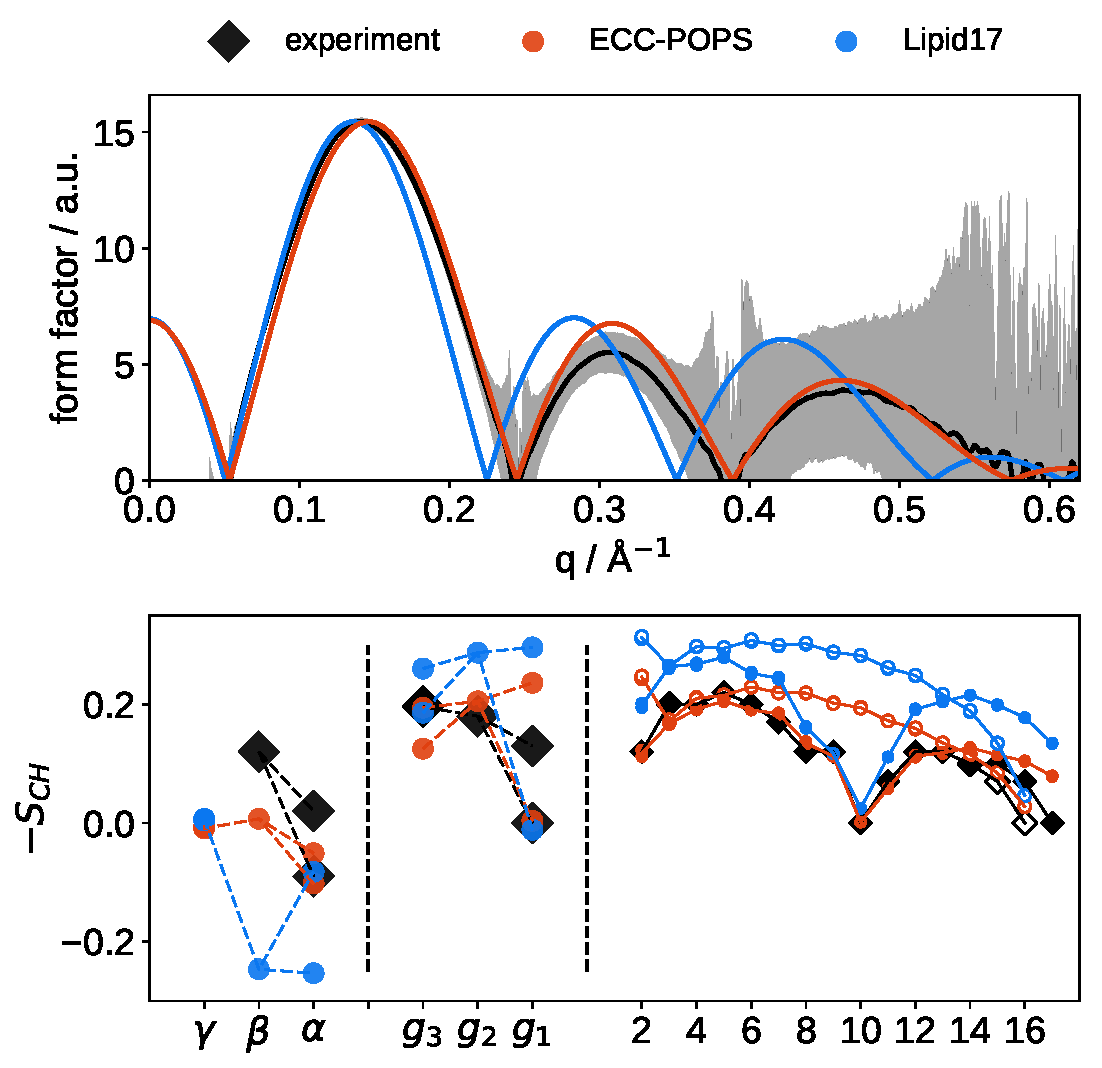
\includegraphics[width=\figwidth]{../img/ecc_pops/Order-parameters_form-factors_exp-L17-ECC-lipids.pdf}
  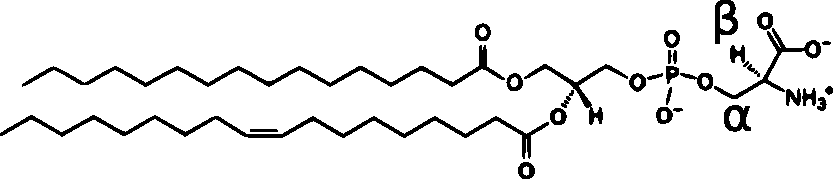
\includegraphics[width=\figwidth]{../img/ecc_pops/pops_chemfig.pdf} 
\hfill
  \caption{\label{simVSexpNOions_POPS} 
    \textbf{Top:} X-ray scattering form factors from simulations with Lipid17/Dang \citep{lipid17-future, dang2006} and 
    the ECC-POPS/ECC-ions \cite{martinek17, Pluhackova2016} compared with experiments~\citep{kucerka14} at 298~K. 
    \textbf{Middle:} Order parameters of POPS head group, glycerol backbone and acyl chains  
    from simulations with the Lipid17 \citep{lipid17-future} and the ECC-POPS models 
    compared with experiments at 298~K. \citep{NMRlipidsIV}
    Open/closed symbols are used for palmitoyl/oleoyl chains of POPS. 
    \textbf{Bottom:} The chemical structure of POPS and the labeling of the carbon segments. 
  }  
  \todo{J: flip the chemical structure so that it agrees with the left-to-right reading of the plot.} \\
\end{figure} 


The Lipid17/Dang simulation give larger acyl chain order parameters and smaller area per molecule than the
experimental values (Fig. \ref{simVSexpNOions_POPS} and table \ref{tab:apls}),
indicating that this simulation predicts too dense POPS lipid bilayer. This is also in line with
the discrepancy observed in the X-ray form factor between this simulation and experiment (Fig. \ref{simVSexpNOions_POPS}).
In previous study \cite{NMRlipidsIV}, the Lipid17 force field with {\AA}qvist ions~\cite{aqvist90}
gave a larger area per molecule (57 \AA$^2$) for POPS being closer to the experimental value,
which is probably due to the weaker counterion binding affinity of {\AA}qvist ions.
However,  {\AA}qvist ions exhibit artificial aggregation of ions at larger salt concentrations \cite{kohagen16, chen07, NMRlipidsIV}.
Therefore, the Dang ions with more realisitic bulk properties are used here to analyze the effect of ECC to the properties of POPS lipid bilayer. 
The ECC-POPS simulation gives a good agreement with the X-ray scattering form factors and experimental
acyl chain order parameters (see Fig.~\ref{simVSexpNOions_POPS}), indicating the the bilayer dimensions and acyl chain
conformations are well described by the force field. The area per lipid from ECC-POPS simulation is slightly
smaller than the value reported from SDP model \cite{kucerka14} (table \ref{tab:apls}), but the values
are within each others error bars. 


% In order to obtain the area per lipid from experiments, modeling is used on top of the scattering factors \citep{kucerka14}. 
%In ocntrast, this property is easily extracted directly from simulations with flat phospholipid bilayers. 
%We compare the values from experiments and simulations in Table~\ref{tab:apls}. 
%While the agreement between the scattering form factors from the simulation of a pure POPS bilayer and experiment 
%are excellent (Fig.~\ref{simVSexpNOions_POPS}), there is a non-negligible difference between the values of the area per lipid in Table~\ref{tab:apls}. 
%Since both values are derived from the scattering form factors through modeling of the electron density of the bilayer,
%we cannot decide, which of the values is more reliable. 

\begin{table}[tb!] 
\centering
  \caption{Area per lipid (APL) of POPS bilayers from simulations with different force fields at 298~K with \ce{Na^+} counterions. \label{tab:apls} } 
  \begin{tabular}{l|c } 
    \multicolumn{2}{c}{POPS} \\
    model          & APL / Å$^2$    \\ 
    \hline 
    Lipid17/Dang              & 53.5$\pm$ 1.7   \\ 
%    Lipid17/ff99              & 57.9$\pm$ 1.7   \\ 
%    \hline 
    ECC-POPS/ECC-ions         & 59.8$\pm$ 1.8   \\ 
%    \hline 
    experiment (SDP model) \citep{kucerka14} & 62.7$\pm$ 1.3  \\ 
%    \hline 
  \end{tabular} \\
\end{table} 

Despite the success in simulating bilayer dimensions and acyl chain conformations,
lipid force fields have typically problems in capturing the correct glycerol backbone and
headgroup order parameters and conformations \cite{botan15,ollila16,NMRlipidsIV}.
This is the case also for Lipid17 POPS simulations, where the headgroup and glycerol backbone
order parameters are quite far from experimental values with both Dang (Fig. \ref{simVSexpNOions_POPS})
and {\AA}qvist \cite{NMRlipidsIV} ions. The values from ECC-POPS simulation are closer,
but not in full agreement with experiments (Fig. \ref{simVSexpNOions_POPS}).
Especially, the experimentally observed more negative values of the $\beta$-carbon
and the larger forking (difference of order parameters between hydrogens attached to the
same carbon \cite{ollila16}) of the $\alpha$-carbon in POPS than in POPC \cite{NMRlipidsIV}
are not reproduced by neither of the models here. These differences are previously related
to a more rigid structure of PS headgroup and the stiffness of the C$_\alpha$-C$_\beta$-C$_\gamma$-O$_\gamma$
dihedral, which is \todo{the dihedral should be plotted and sentence finished.}

%The head group order parameters $\alpha$ and $\beta$ are highly relevant for this work,
%as they are being used in the electrometer concept \cite{altenbach84, catte16, melcr18}.
%For POPC in pure water, the order parameter $\beta$ agrees well with the experiment, while the order parameter $\alpha$ is somewhat lower. 

In conclusion, the ECC-POPS model reproduces the lipid bilayer dimensions and
acyl chain conformations in good agreement with experiments, but has room for
improvement in the glycerol backbone and headgroup region. Therefore,
its structural accuracy is in the same level as in other state-of-the-art
lipid force fields \cite{botan15, ollila16, Pluhackova2016, NMRlipidsIV}.
 
 
\subsection{Counterion binding affinity and interactions between PC and PS head groups}

\begin{figure}[tbp!] 
  \centering 
  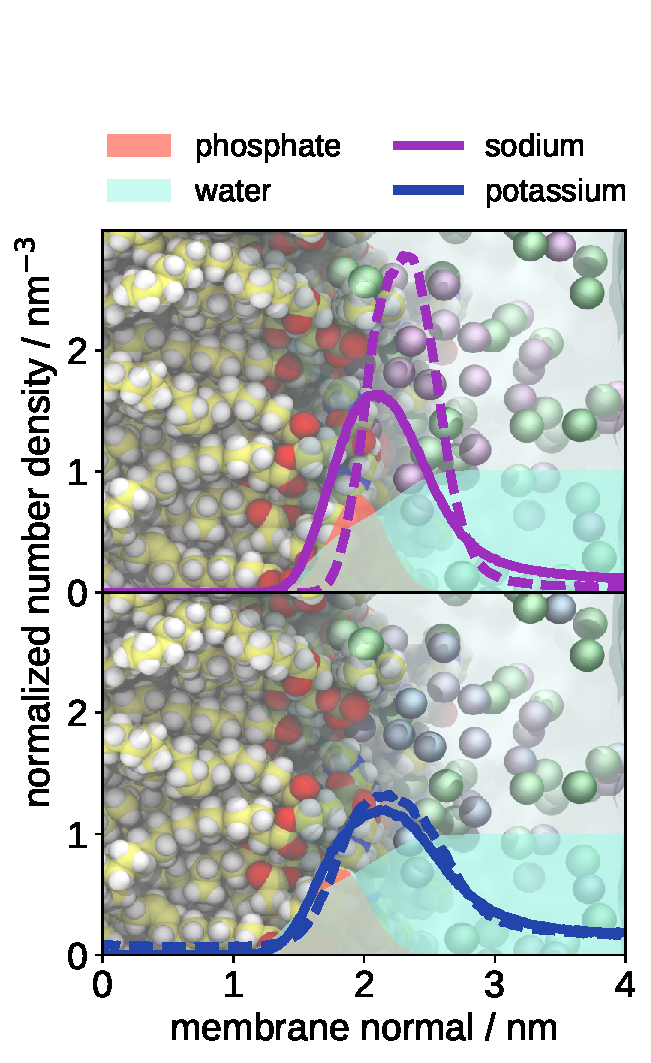
\includegraphics[height=\figheight]{../img/ecc_pops/density_profiles_na-k-counterions_wat_phos_compar_purePOPS_ecclipids-lipid17.pdf}
  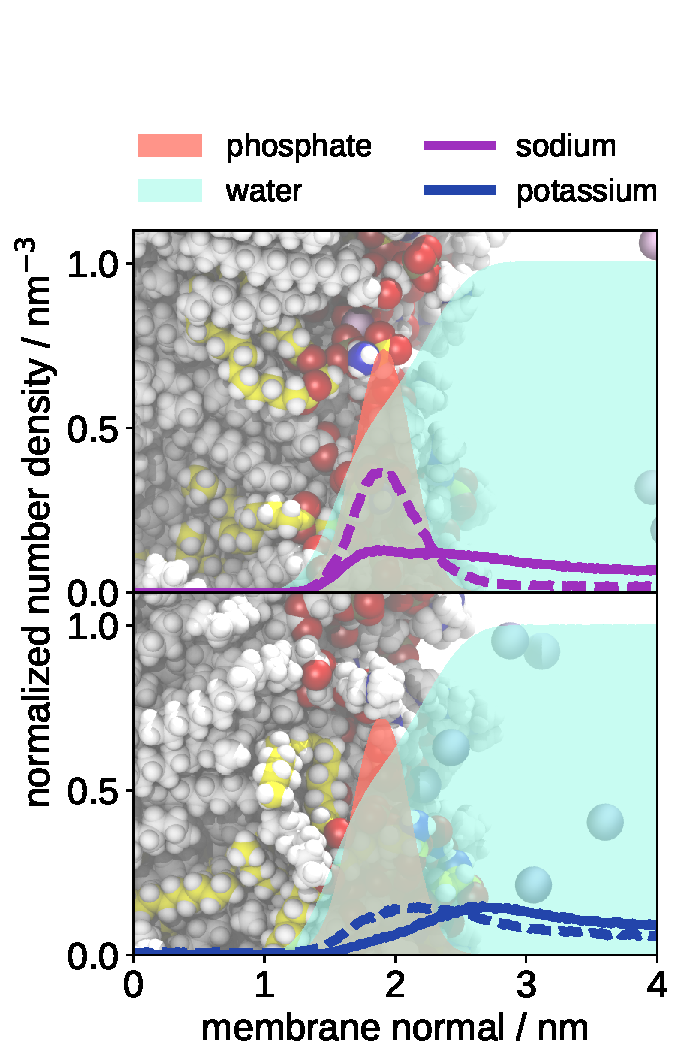
\includegraphics[height=\figheight]{../img/ecc_pops/density_profiles_na-k-counterions_wat_phos_compar_5PC-1PS_ecclipids-lipid17.pdf}
  \caption{\label{fig:POPS-counterions-dens}
    Number density profiles of \ce{K^{+}} and \ce{Na^{+}} counterions along the membrane normal axis
    in ECC-lipids (solid lines) and Lipid17/Dang (dashed lines) simulations of pure POPS (left) or POPC:POPS (5:1, right) bilayers.  
    The density profiles of phosphate groups and water are divided by 4 and 100, respectively.  
}
\end{figure} 
Binding affinity of monovalent ions to lipid bilayers depends strongly on
force field parameters \cite{catte16,NMRlipidsIV},
which is the case also here as the sodium counterion binding affinity to
POPS lipid bilayer is stronger in Lipid17/ Dang simulation than in
ECC-POPS simulation (Fig. \ref{fig:POPS-counterions-dens}).
The cation binding affinities to lipid bilayers in simulations have been previously evaluated
against experiments using the order parameters of $\alpha$ and $\beta$ carbons in the
phosphatidylcholine (PC) lipid headgroup (see Fig.~\ref{fig:chemstruct_pc_ps} for the labeling) \cite{catte16,melcr18,NMRlipidsIV},
which decrease proportionally to the bound charge according to the ''electrometer concept'' \citep{seelig87}.
Althought the response of PS lipid headgroup order parameters to the bound charge is also systematic,
it is less well undestood and the addition of cations may cause phase transitions in negatively charged
bilayers \cite{feigenson86,mattai89,roux91,roux90}. Therefore, the cation binding affinity to bilayers with
PS lipids has been evaluated measuring the PC headgroup order parameters from POPC:POPS (5:1)
mixtures\cite{roux90,NMRlipidsIV}.
Following our previous work \cite{NMRlipidsIV}, we evaluate the counterion binding affinity
to lipid bilayer in simulations containing PS using two different approaches.

% The situation is more complicated for lipid bilayers containing
%PS lipids, for which there is no ion-free reference state due to the presence of counterions.

%Unlinke in pure PC bilayers,
%Interpreting the changes of the head group order parameters of 
%mixed PC:PS lipid bilayers 
%from both simulations and experiments
%is complicated by the presence of counterions. \cite{NMRlipidsIV}

\begin{figure}[tb!] 
  \centering 
  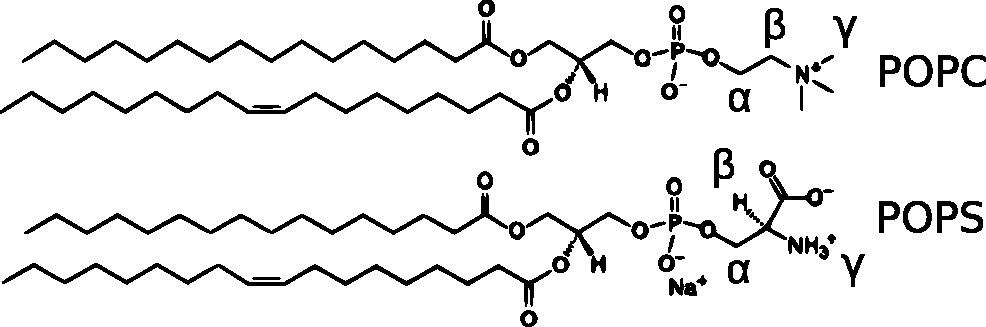
\includegraphics[width=\figwidth]{../Fig/lipids_chemfig_POPC_POPS.pdf} 
  \caption{ \label{fig:chemstruct_pc_ps} 
            The chemical structure of POPC and POPS 
            including the labeling of the carbon segments
            used in the measurements of order parameteres. 
          }
          \todo{The POPS structure and labeling is already in figure \ref{simVSexpNOions_POPS}.
            The POPC structure and labeling could be added on top of the new version of figure \ref{fig:delta_ordPar_NaCl_PC-PS_mix} with only PC,
            where PC results occur in the first time, and this figure could be removed.} \\
          \todo{$\gamma$ carbon of POPS is the COO- minus carbon. The $\gamma$ label should be moved there.}
\end{figure} 
 
The head group and acyl chain order parameters within ECC-lipids
are in general in a good agreement with the experimental values 
as shown in Fig. \ref{simVSexpNOions_POPS}. 
The acyl chain order parameters in particular agree with the experimental data within error bars.
The order parameters of the head groups are at an accuracy comparable to 
other currently available classical models of lipids \citep{botan15, catte16, Pluhackova2016, nmrlipids_proj4}. 
In particular, ECC-POPS is closer to the experimental order parameters 
than Lipid17 with either Dang \cite{smith94,chang1999,dang2006} 
or ff99 ions \citet{aqvist90}. 

%This was demonstrated for a bound positive charge in simulations with POPC and 
%cationic surfactants or aquaeous cations employing the ECC-POPC model \cite{melcr18}.
%In this work, we will use the electrometer concept also for a bound negative charge 
%using PS lipids as negatively charged surfactants. \cite{roux90} 

%is the
%is not generally agreed on between simulations 
%\citep{bockmann03,sachs04,berkowitz06,cordomi09}
%and experiments 
%\citep{cevc90,tocanne90,hauser76,herbette84,uhrikova08}.
%We attempted to find a model, 
%which would successfully interpret the experiments on binding of \ce{Na^+}
%to neutral and negatively charged phospholipid bilayers \citep{akutsu81, roux90} 
%in our works \citep{catte16, NMRlipidsIV}.
%After testing the currently available force fields for phospholipids,
%we concluded
%that the interactions are generally overestimated in magnitude in almost all models 
%but Lipid14 (PC) \citep{dickson14}, resp. Lipid17 (PS) \citep{lipid17-future}. 
%This model yields a semi-quantitative agreement with the experimentally measured small changes of the order parameters \cite{catte16}
%when used with the model of ions by \citet{aqvist90}. 
%However, when used with a more accurate model of ions by \citet{Pluharova2014, martinek17},
%the model overestimates the binding affinity of \ce{Na^+}
%measured with lipid electrometer concept. \citep{melcr18}
%In total, these results suggest that improvements 
%in the lipid parameters are required for more accurate interactions even with monovalent cations. 
%\citep{catte16, melcr18, NMRlipidsIV}


\begin{figure*}[!tbp] 
  \centering 
  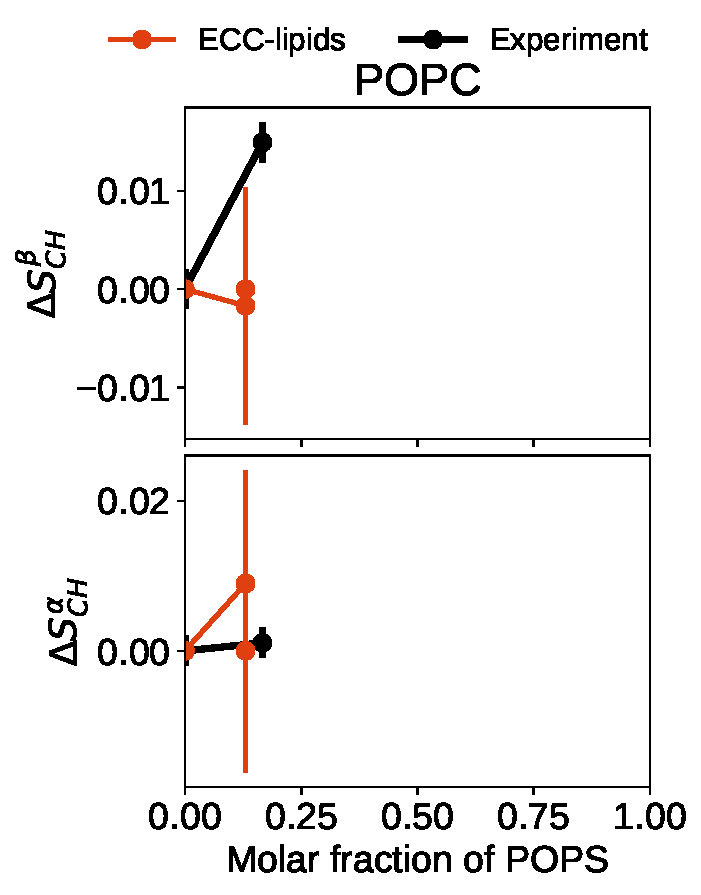
\includegraphics[height=\figheightsmall]{../Fig/order_parameters_changes_A-B_PC-PS_mix_POPC_nacl.pdf} 
  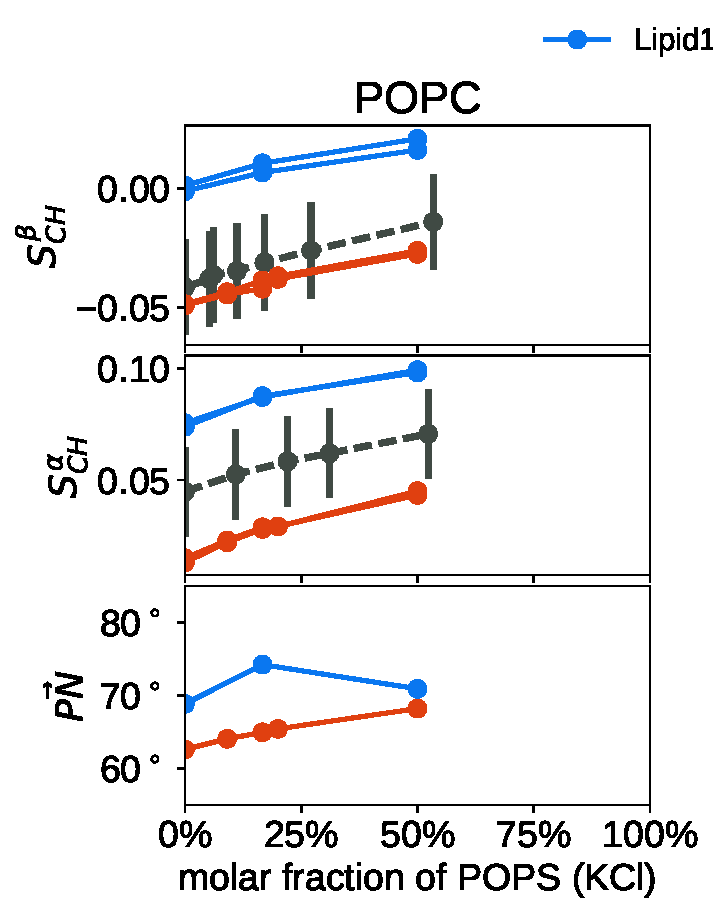
\includegraphics[height=\figheightsmall]{../Fig/order_parameters_changes_A-B_PC-PS_mix_POPC_kcl.pdf} 
  \caption{\label{fig:delta_ordPar_NaCl_PC-PS_mix_PC} 
    The POPC head group order parameters and the P--N vector angle
    with respect to the membrane normal as a function of POPS content in a bilayer
    from ECC-lipids and Lipid17/Dang simulations with \ce{Na^+} (top) and \ce{K^+} (bottom) counterions.
    Experimental order parameter values are from Ref. \citenum{scherer87}
    and the signs from Ref. \citenum{ferreira16} (only \ce{Na^+} counterions, but shown also in bottom plots).
  }
\end{figure*} 


\begin{figure*}[!tbp] 
  \centering 
  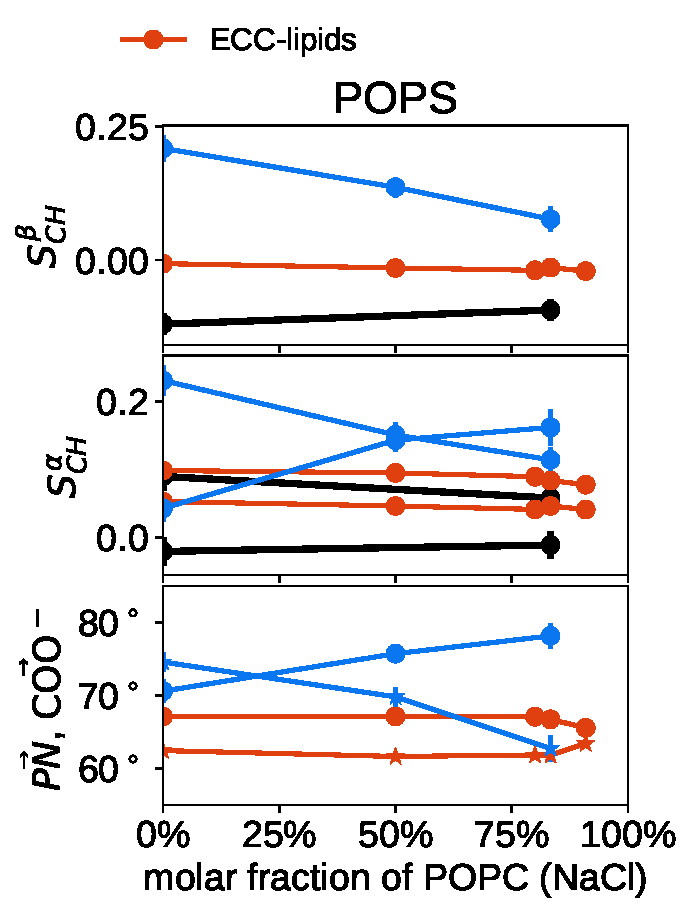
\includegraphics[height=\figheightsmall]{../Fig/order_parameters_changes_A-B_PC-PS_mix_POPS_nacl.pdf} 
  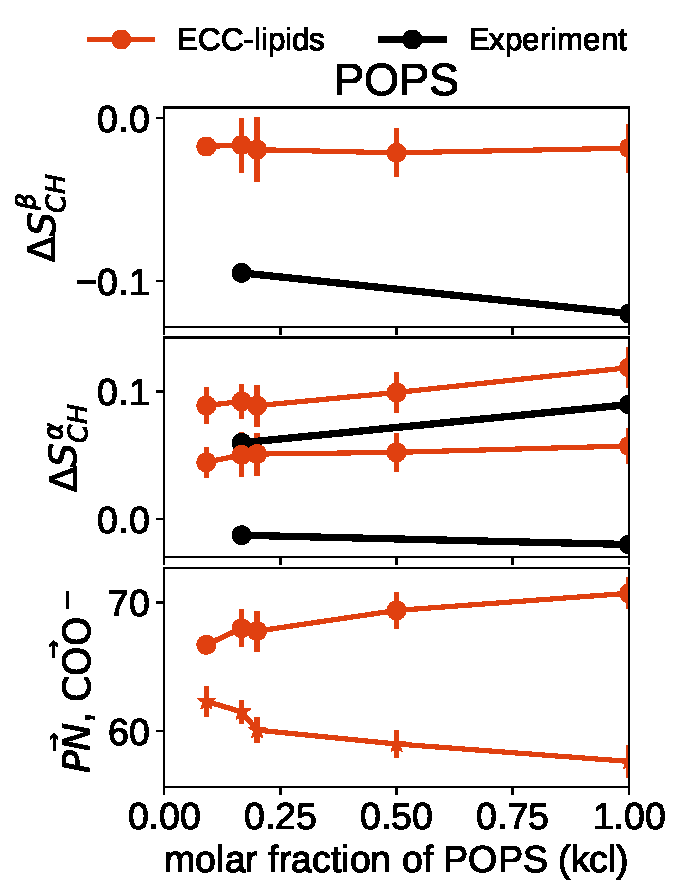
\includegraphics[height=\figheightsmall]{../Fig/order_parameters_changes_A-B_PC-PS_mix_POPS_kcl.pdf} 
  \caption{\label{fig:delta_ordPar_NaCl_PC-PS_mix_PS} 
    The POPS head group order parameters, the P--N and C$_\beta$--C$_\gamma$ vector angles (stars)
    with respect to the membrane normal as a function of POPC content in a bilayer
    from ECC-lipids and Lipid17/Dang simulations with \ce{Na^+} (top) and \ce{K^+} (bottom) counterions.
    Experimental order parameter values and signs for pure POPS are from Ref. \citenum{NMRlipidsIV} and values
    for POPC:POPS (5:1) mixture from Ref. \citenum{roux90} (only \ce{Na^+} counterions, but shown also in bottom plots).
    %The underestimated response of ECC-lipids with \ce{Na^+} counterions 
    %is likely due to a still slightly overestimated binding affinity of \ce{Na^+} to the phospholipids,
    %which is corroborated by the series with \ce{K^+} counterions (lower affinity than \ce{Na^+}),
    %where the response is closer to the experiment, which uses only \ce{Na^+} counterions. 
  }
\end{figure*} 


First, we monitor the response of POPC headgroup order parameters to the increasing amount of POPS (Fig.~\ref{fig:delta_ordPar_NaCl_PC-PS_mix}).
According to the electrometer concept, the head group order parameters of PC lipids increase
with the increasing amount of negatively charged PS lipids in experiments, because the headgroup P--N dipole
tilts more parallel to the membrane interface \cite{seelig87,scherer87}.
The trend is observed with both force fields in simulations with \ce{K+} counterions and
in ECC-POPS simulation with \ce{Na+} counterions, but not in Lipid17/Dang ion simulations with \ce{Na+} counterions,
where the order parameters are unchanged or decrease and the P--N vector tilts more perpendicular to the membrane interface.
The result can be explained by the higher binding affinity of sodium in the
Lipid17/Dang ion simulations (Fig~\ref{fig:POPS-counterions-dens}), which
compensates the negative charge of PS lipids at the interface.

Second, we monitor the response of PC headgroup order parameters to the additional
amount of sodium and potassium in POPC:POPS (5:1) mixtures.
In experiments, the addition of K$^+$ ions led to a very modest decrease of the order parameters,
while the decrease was more pronounced with Li$^+$ ions and strongest with divalent Ca$^{2+}$ and Mg$^{2+}$ ions \cite{roux90}.
According to the electrometer concept, the decrease of PC lipid head group order parameters
correlates with the amount of bound cations \cite{akutsu81,altenbach84,seelig87,roux90,catte16,NMRlipidsIV},
thus the binding affinity of the ions to POPC:POPS (5:1) mixtures increase in order K$^{+}$ $<$ Li$^{+}$  $<$ Mg$^{2+}$  $<$ Ca$^{2+}$.
The response of PC headgroup order parameters to the increasing amount of KCl is close to experiments
and the change in P--N vector is negligible in both force fields (Fig. \ref{fig:delta_ordPar_KCl_PCPS}), athought the change of the $\alpha$-carbon
order parameter may be slightly overestimated by the Lipid17/Dang simulations. This could be
explained by the slightly deeper penetration of potassium into the bilayer (Fig. \ref{fig:POPS-counterions-dens}).
Because experimental data with the additional amount of sodium in POPC:POPS (5:1) mixture was not available,
we compared the simulation results to the experimental data with the additional amounts of
lithium and potassium ions, which should give the lower and upper bounds to the sodium binding
affinity (Fig. \ref{fig:delta_ordPar_NaCl_PCPS}). The PC headgroup response to the additional
amount of sodium is clearly overestimated by the Lipid17/Dang simulation and
the response in ECC-POPS simulations is probably too close to the experimental results for lithium.
In conclusion, the results suggest that the sodium binding affinity (Fig. \ref{fig:POPS-counterions-dens}) and
the tilting of P--N vector more perpendicular to the membrane surface (Fig. \ref{fig:delta_ordPar_NaCl_PCPS})
are clearly overestimated in Lipid17/Dang simulations and slightly overestimated in ECC-POPS simulations,
while the binding affinity of potassium is better described by both force fields.

%Generally improved behaviour 
%of the POPC and POPS head group order parameters 
%with \ce{NaCl} or \ce{KCl} concentrations 
%was achieved through the combination of models 
%ECC-lipids and ECC-ions \citep{martinek17, kohagen16, Pluharova2014}. 
%Simulations with these models 
%reveal a good agreement with the NMR experiments 
%for both neutral and negatively charged membranes.
%The results are plotted for \ce{NaCl} in Fig. \ref{fig:delta_ordPar_NaCl_PCPS}, 
%and for \ce{KCl} in Fig. \ref{fig:delta_ordPar_KCl_PCPS}. 


%The order parameters of the PS head groups including their changes with the content of PC lipids
%are challenging to capture correctly in classical MD simulation models. \cite{NMRlipidsIV}
%From such a perspective,
%the changes of the PS head group order parameters from ECC-lipids 
%with \ce{Na+}, and also \ce{K+}, counterions 
%agree comparably well to the experimental measurements
%(Fig.~\ref{fig:delta_ordPar_NaCl_PC-PS_mix}). 
%Interestingly enough, 
%although the Lipid17 model performed well with \ce{K+} counterions 
%for the PC head group order parameter changes,
%it does not agree in the equivalent changes in PS head groups
%pointing at non-negligible effects of even relatively weakly binding cations 
%on the structure of negatively charged lipids. 

%Despite the great improvements in the overall structure of ECC-POPS 
%and its response to PC lipids and counterions,
%there is still a large room for improving it
%to agree with the experimental measurements. 

%\subsection{Molecular interaction and binding affinities of K$^+$ and Na$^+$ cations to mixed POPC:POPS (5:1) membrane} 
%\label{sec:K_Na_added} 
 
 
\begin{figure}[tbp!] 
  \centering 
  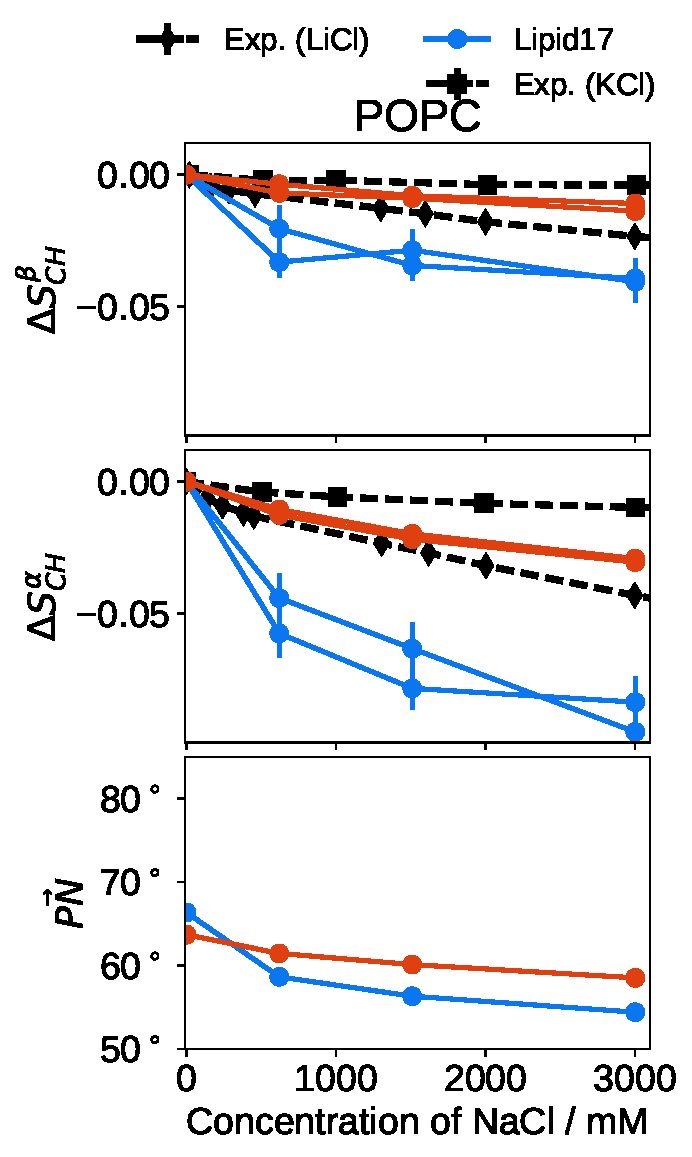
\includegraphics[height=\figheight]{../img/ecc_pops/order_parameters_changes_ecc-lip_L14_A-B-PN-COO_POPC_nacl.pdf} 
  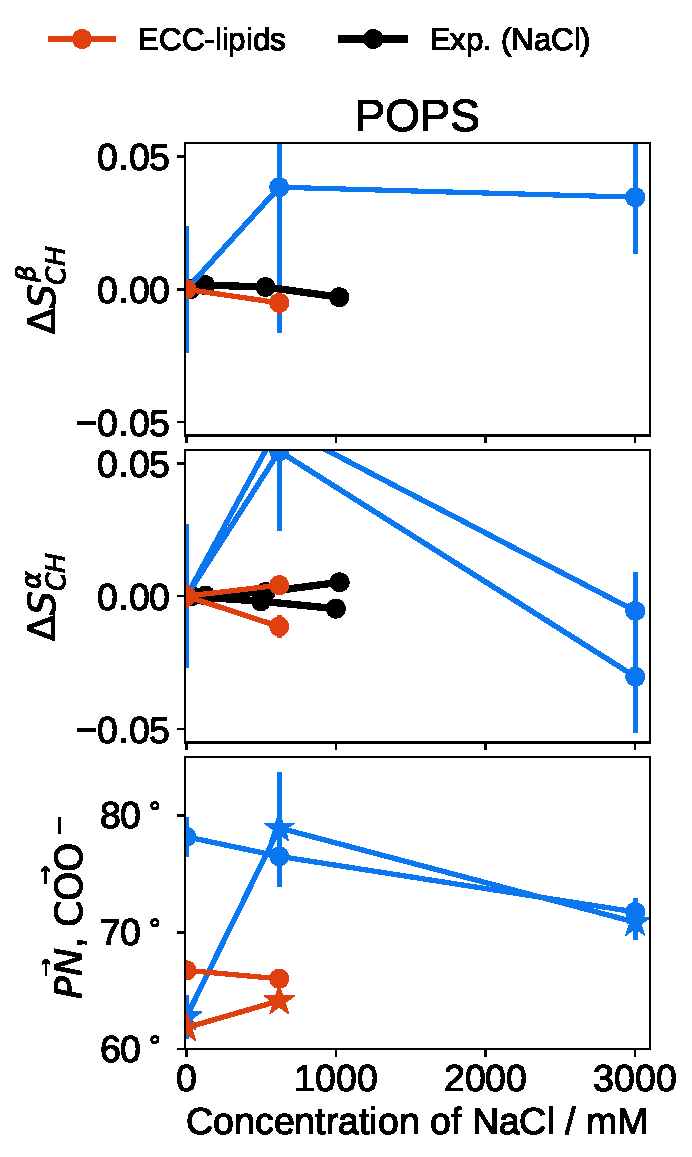
\includegraphics[height=\figheight]{../img/ecc_pops/order_parameters_changes_ecc-lip_L14_A-B-PN-COO_POPS_nacl.pdf} 
  \caption{\label{fig:delta_ordPar_NaCl_PCPS} 
    Changes of the head group order parameters, and the angles of P--N and C$_\beta$--C$_\gamma$ (stars) vectors
    with respect to the membrane normal of POPC (left) and POPS (right) in a POPC:POPS (5:1) bilayer 
    as a function of \ce{NaCl} concentration from ECC-lipids and Lipid17/Dang simulations at 298 K.
    The y-axis for the $\alpha$-carbon results of POPS (middle right) is transferred
    with the same value for both order parameters such that the lower order
    parameter value from pure POPS is at zero to correctly illustrate the significant forking.
    Because experimental data with \ce{NaCl} is not available for POPC, the data for KCl and \ce{LiCl} (dashed line, left)
    are shown as lower and upper bounds for the response to \ce{NaCl}, respectively.
    The magnitudes of experimental order parameters are from Ref. \citenum{roux90} and signs from Ref. \citenum{ferreira16}.
    %which has a lower affinity to phospholipid bilayers compared to \ce{LiCl} \citep{roux90}. 
    %The orientation of the \ce{COO^-} group is defined as 
    %the connector from the $\beta$ carbon to the carbon in \ce{COO^-} (stars, bottom right). 
  }
  \end{figure} 


\begin{figure}[tbp!] 
  \centering 
  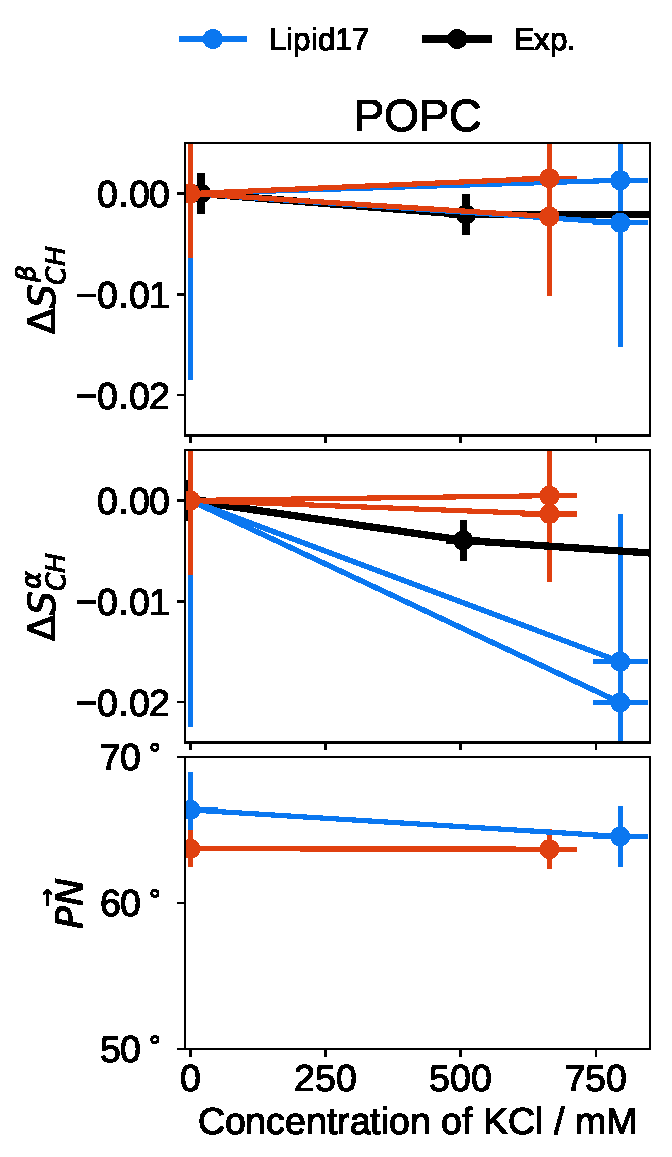
\includegraphics[height=\figheight]{../img/ecc_pops/order_parameters_changes_ecc-lip_L14_A-B-PN-COO_POPC_kcl.pdf} 
  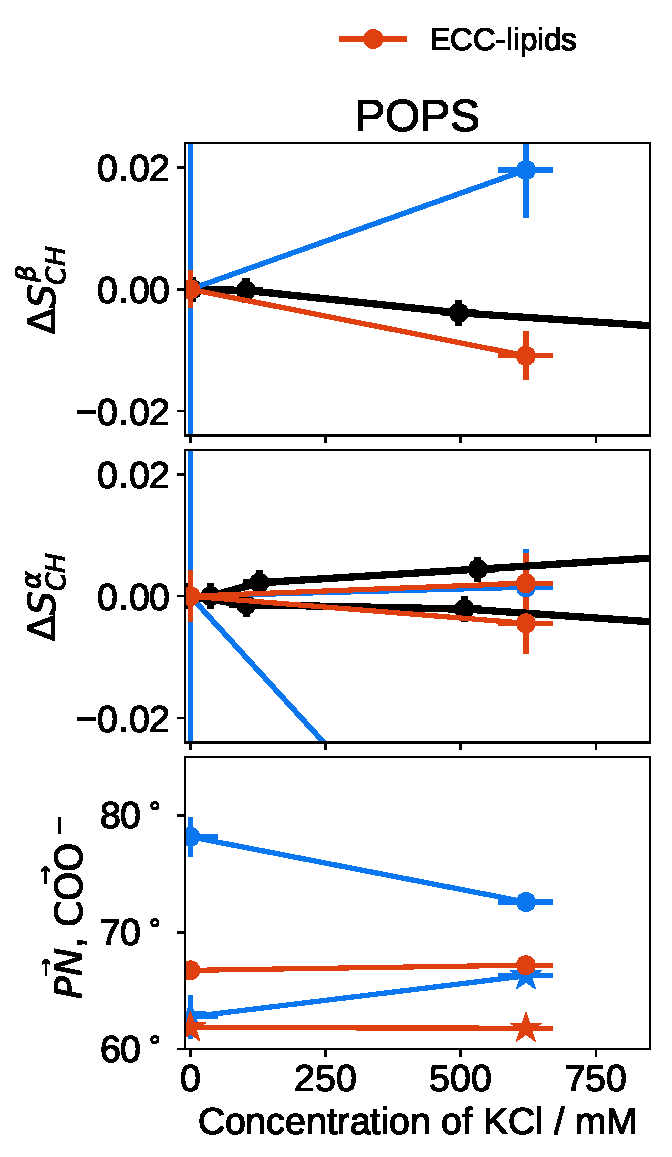
\includegraphics[height=\figheight]{../img/ecc_pops/order_parameters_changes_ecc-lip_L14_A-B-PN-COO_POPS_kcl.pdf} 
  \caption{\label{fig:delta_ordPar_KCl_PCPS}
    Changes of the head group order parameters, and the angles of P--N and C$_\beta$--C$_\gamma$ (stars) vectors 
    with respect to the membrane normal of POPC (left) and POPS (right) in a POPC:POPS (5:1) bilayer 
    as a function of \ce{KCl} concentration from ECC-lipids and Lipid17/Dang simulations 
    compared with experimental values from Ref. \citenum{roux90} (signs from Ref. \citenum{ferreira16}) at 298 K.
    The y-axis for the $\alpha$-carbon results of POPS (middle right) is transferred
    with the same value for both order parameters such that the lower order
    parameter value from pure POPS is at zero to correctly illustrate the significant forking.
  }
\end{figure} 
 
% This§: 
% Other models do not yield good reponse, but
% ECC-lipid describe the changes well
% => Elect. polar. necessarry.
% 
The changes of POPS headgroup order parameters are almost negligible in experiments with increasing POPC fraction in bilayer
or monovalent ion concentration in solvent
(Figs. \ref{fig:delta_ordPar_NaCl_PCPS}, \ref{fig:delta_ordPar_KCl_PCPS} and \ref{fig:delta_ordPar_NaCl_PC-PS_mix}).
%while calcium leads to relatively large changes with low concentrations followed by a rapid saturation below 100mM (Fig. \ref{fig:delta_ordPar_CaCl_PCPS}) \cite{scherer87,roux90}.
%The interaction with \ce{K^+}, which binds very weakly to both neutral and negatively charged membranes, 
%renders a qualitatively different response of the order parameter $S^\beta$ in POPS 
%in the mixed negatively charged bilayers compared to the neutral bilayers. 
%While the order parameter $S^\beta$ increases for both \ce{Na^+} and \ce{Ca^{2+}},
%it decreases in the presence of \ce{K^+}
%(\ce{KCl}:  Fig.~\ref{fig:delta_ordPar_KCl_PCPS}, 
% \ce{NaCl}: Fig.~\ref{fig:delta_ordPar_NaCl_PCPS}, and
%\ce{CaCl2}: Fig.~\ref{fig:delta_ordPar_CaCl_PCPS}). 
In Lipid17/Dang simulations, the changes of POPS headgroup order parameters with increasing amount of POPC
are overestimated, which is also related to the changes in the orientations of the P--N and C$_{\beta}$--C$_{\gamma}$
vectors (Fig. \ref{fig:delta_ordPar_NaCl_PC-PS_mix}). The overestimation of the order parameter changes
upon increasing amount of POPC in a bilayer 
was also observed in previous simulations with other force fields \cite{NMRlipidsIV}, but not in
ECC-POPS simulation, where also the changes in the PS headgroup orientation are more modest (Fig. \ref{fig:delta_ordPar_NaCl_PC-PS_mix}).
The POPS headgroup orientation and order parameters are more sensitive also to the additional amount
of sodium and potassium in Lipid17/Dang simulations, while dependence is weaker and closer to experiments
in ECC-POPS simulations (Figs. \ref{fig:delta_ordPar_NaCl_PCPS} and \ref{fig:delta_ordPar_KCl_PCPS}).
%In contrast, ECC-lipids with ECC-ions capture the different response 
%of the order parameters $S^{\beta}$, $S^{\alpha _1}$ and $S^{\alpha _2}$ in POPS 
%to various concentrations of \ce{NaCl} and \ce{KCl} in a good agreement with the experiments
%(\ce{KCl}:  Fig.~\ref{fig:delta_ordPar_KCl_PCPS}, 
% \ce{NaCl}: Fig.~\ref{fig:delta_ordPar_NaCl_PCPS}). 
%Such a dramatic improvement in the structural parameters 
%demonstrates that including electronic polarization in phospholipids is crucial 
%even for interactions with soft cations like \ce{K^+}. 

% This§: 
% adsorption and affinities of Na and K to PC:PS memb
% from densities and rel.surf.excess
% 
%in  Fig.~\ref{fig:POPS-counterions-dens} (only counterions)
%and Fig.~\ref{fig:nacl-dens_PCPS}        (additional salt concentrations), 
%
The influence of negatively charged PS on the counterion binding affinity can
be estimated by comparing the relative surface excesses with respect to water, $\Gamma ^{w} _{\rm ion}$,
between POPC:POPS (5:1) mixture and pure POPC \cite{melcr18}.
%Such a quantity compares the adsorption of ions to the adsorption of water molecules at an interface 
%without the necessity of defining a Gibbs dividing surface. \citep{melcr18, chattorajBOOK}
The value of $\Gamma ^{w} _{\rm Na}=-0.11 \pm 0.01 \mathrm{nm}^{-2}$ for 1 M sodium in pure ECC-POPC
simulation was reported in the previous work \cite{melcr18}.
The presence of $\sim$17\$ POPS in POPC bilayer increases the
%relative surface excess of sodium with respect to water from negative
value to $\Gamma ^{w} _{\rm Na}=0.092 \pm 0.005 \mathrm{nm}^{-2}$ 
for 0.621 M sodium, while value for potassium remains negative,
$\Gamma ^{w} _{\rm K}=-0.123 \pm 0.005 \mathrm{nm}^{-2}$ in POPC:POPS (5:1) mixture (Fig. \ref{fig:nacl-dens_PCPS}).
As discussed above, the sodium binding to POPC:POPS (5:1) mixture may be slightly overestimated also in
ECC-lipids simulations. The response of headgroup order parameters to the addition of NaCl are
slightly overestimated also in ECC-POPC simulations (Fig 3 in Ref. \citenum{melcr18}),
suggesting that similar small overestimation of sodium binding may also occur to a pure POPC bilayer.
Therefore, the overestimation may arise from the sodium interactions with PC headgroup and
increase in binding affinity due to PS lipids would not be affected.
%Interestingly enough, \ce{K^+} maintains negative values of $\Gamma^{w}_{K}$ even for the negatively charged PC:PS~(5:1) bilayer.
%This is also evident from the density plots in  Fig.~\ref{fig:nacl-dens_PCPS}
%showing that the density profile of \ce{K^+} along the membrane normal 
%decays clearly faster towards the membrane centre compared to the density of water. 
%In contrast, the density profile of \ce{Na^+} has a shoulder 
%at the region of the phosphate groups,
%which demonstrates that sodium cations adsorb weakly to the membrane interface compared to the aquaeous solution
%by yielding a small positive value of $\Gamma^{w}_{Na}$.

In conclusion, applying ECC to Amber Lipid17 POPS force field parameters improves its
interactions with both monovalent ions and POPC headgroups when compared with the NMR order parameter data.
However, further optimization may be needed to fully reproduce the interactions between lipids and
sodium ions.


\subsection{Molecular interaction and binding affinities of \ce{Ca^{2+}} cations to mixed POPC:POPS (5:1) membrane} 
\label{section:lip-ion_ca}

%The headgroup order parameters of PC lipids decrease more upon addition of \ce{CaCl2}
%in POPC:POPS (5:1) mixtures than in pure PC bilayers due to the higher calcium binding
%affinity to the negatively charged lipid bilayers \cite{akutsu81,altenbach84,roux90,NMRlipidsIV}.
Our recent work demonstrates that the POPC headgroup order parameters measured
from POPC:POPS (5:1) mixture as a function of CaCl$_2$ concentration \cite{roux90}
can be used to evaluate the calcium binding affinity to lipid bilayers containing PS lipids \cite{NMRlipidsIV}.
The decrease of the PC headgroup order parameters in this mixture upon addition of \ce{CaCl2} 
were overestimated by the Lipid17/Dang simulations (also shown in Fig.~\ref{fig:delta_ordPar_CaCl_PCPS})
and all the other tested force fields, except CHARMM36 with the recently introduced NBfix for calcium \cite{kim16},
which underestimated the headgroup order parameter response.
In ECC-lipids simulations, the headgroup responses are in better agreement with experiments (Fig.~\ref{fig:delta_ordPar_CaCl_PCPS}),
indicating that the lower binding affinity than in Lipid17/Dang simulations is more realistic (Fig.~\ref{fig:cacl-dens_PCPS}).
%However, the steep decrease of the order parameters at low calcium concentrations,
%observed especially in negatively charged bilayers \cite{borle85,macdonald87,roux90},
%may not be fully captured by the ECC-lipids simulations.
The increased calcium binding affinity to bilayers containing PS lipids is illustrated in
ECC-lipids simulations by the increasing relative surface excess of calcium with respect to water from
$\Gamma^{w}_{Ca} = 0.06\mathrm{nm^{-2}}$ for pure POPC bilayer with 350 mM CaCl$_2$ \cite{melcr18}
to $\Gamma^{w}_{Ca} = 0.24\mathrm{nm^{-2}}$ for the POPC:POPS (5:1) bilayer with 409 mM CaCl$_2$.

%The binding of calcium cations to the phospholipid bilayer is shown 
%in the density profiles of \ce{Ca^{2+}}, \ce{Na^+} counterions 
%and also \ce{Cl^-} ions in Fig.~\ref{fig:cacl-dens_PCPS}. 
%Clearly, after accounting for the electronic polarizability, 
%the population of the cations at the membrane interface is significantly diminished. 

\begin{figure}[tbp!] 
  \centering 
  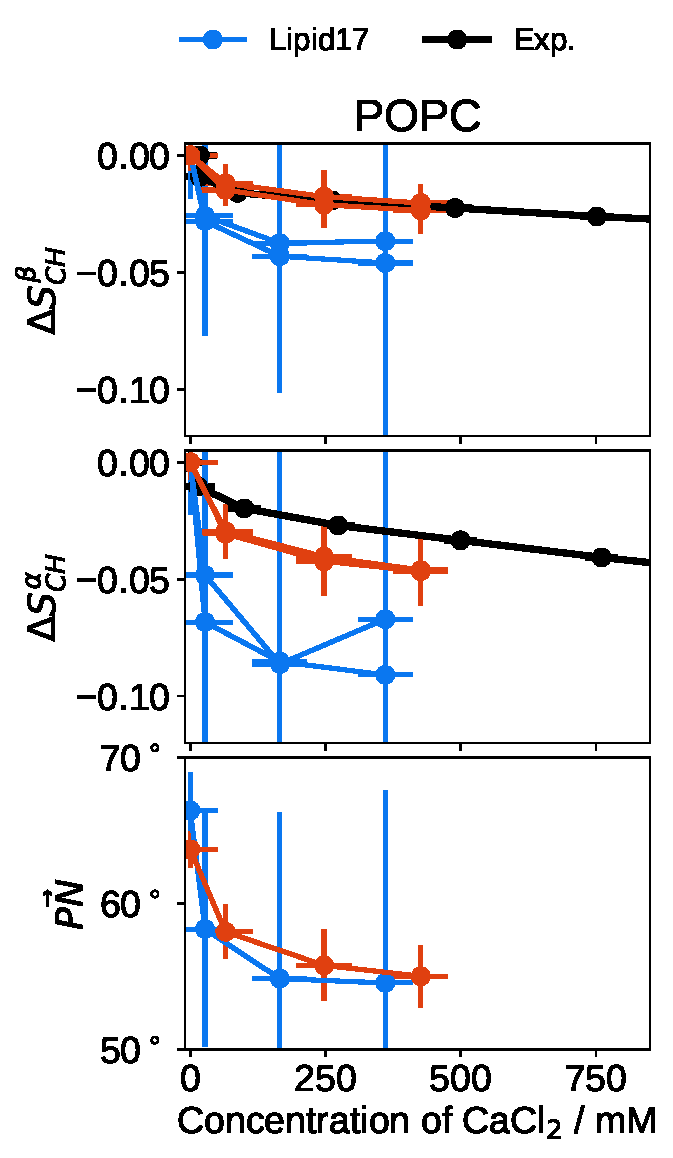
\includegraphics[height=\figheight]{../img/ecc_pops/order_parameters_changes_ecc-lip_L14_A-B-PN-COO_POPC_cacl.pdf} 
  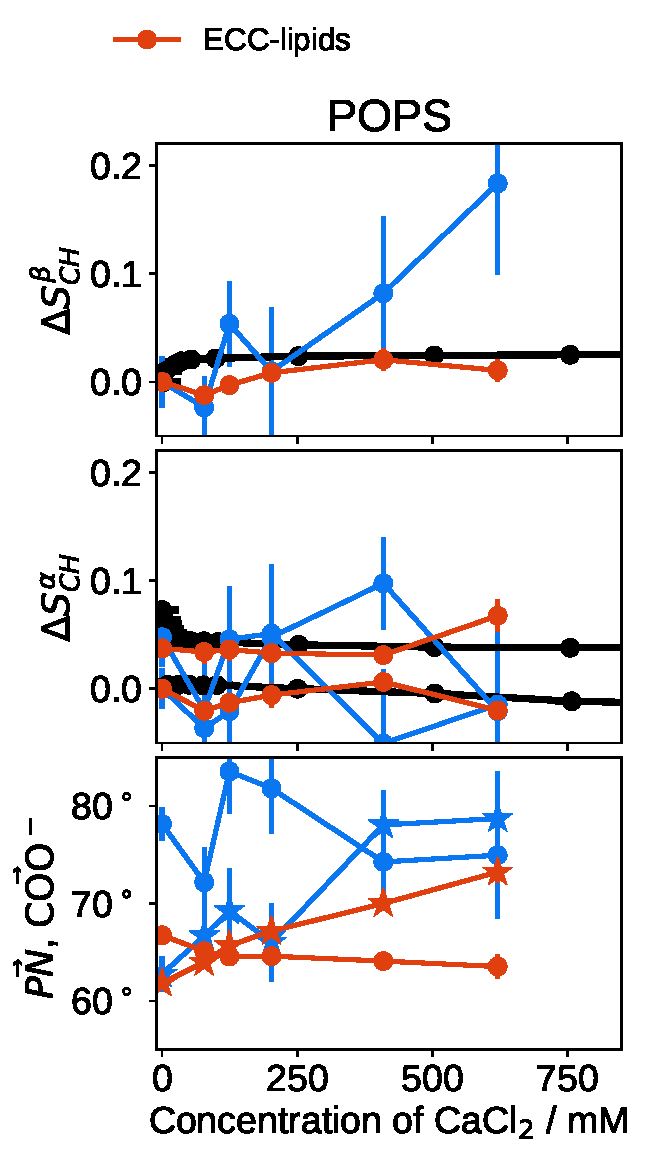
\includegraphics[height=\figheight]{../img/ecc_pops/order_parameters_changes_ecc-lip_L14_A-B-PN-COO_POPS_cacl.pdf} 
  \caption{\label{fig:delta_ordPar_CaCl_PCPS} 
    Changes of the head group order parameters, and the angles of P--N and C$_\beta$--C$_\gamma$ (stars) vectors 
    with respect to the membrane normal of POPC (left) and POPS (right) in a POPC:POPS (5:1) bilayer 
    as a function of \ce{CaCl} concentration from ECC-lipids and Lipid17/Dang simulations 
    compared with experimental values from Ref. \citenum{roux90} (signs from Ref. \citenum{ferreira16}) at 298 K.
    The y-axis for the $\alpha$-carbon results of POPS (middle right) is transferred
    with the same value for both order parameters such that the lower order
    parameter value from pure POPS is at zero to correctly illustrate the significant forking.
  }
\end{figure} 

Experimentally measured headgroup order parameters of POPS exhibit a strong dependence
on low CaCl$_2$ concentrations with a rapid saturation below 100 mM \cite{roux90}.
Also these changes were overestimated by the Lipid17/Dang (also shown in Fig.~\ref{fig:delta_ordPar_CaCl_PCPS})
and other tested force fields in our recent work \cite{NMRlipidsIV}, including CHARMM36 with the NBfix correction for calcium
which underestimated the binding affinity.
In ECC-lipids simulations, the changes of the PS headgroup order parameters are not overestimated,
but the strong dependence on low concetrations of CaCl$_2$ is not fully reproduced (Fig.~\ref{fig:delta_ordPar_CaCl_PCPS}).
In addition to the inaccurate interactions between calcium ions and PS headgroup, the potential sources of this
discrepancy include the above observed slight overestimation of \ce{Na^+} counterions and
inaccurate structures of the lipid headgroup (Fig.~\ref{simVSexpNOions_POPS}).

In ECC-lipids simulations, the average orientation of P--N vectors of both POPC and POPS headgroups tilts more perpendicular to the membrane surface
by 11$^\circ$ and  3$^\circ$, respectively, upon addition of 620~mM CaCl$_2$ to POPC:POPS (5:1) mixture (Fig.~\ref{fig:delta_ordPar_CaCl_PCPS}),
suggesting that the PS headgroup orientation is less sensitive to the bound calcium than PC.
On the other hand, the average orientation of the C$_{\beta}$--C$_{\gamma}$ vector PS headgroup
tilts to the opposite direction by $11^\circ$ in the same system.
%the systematic tilting of P--N and C$_{\beta}$--C$_{\gamma}$ vectors 
%to more perpendicular and parallel direction with respect to the membrane interface, respectively,
%is observed upon addition of CaCl$_2$ (Fig.~\ref{fig:delta_ordPar_CaCl_PCPS}).
In Lipid17/Dang simulations, the changes in both headroup orientations and order parameters
are larger and less systematic for the PS headgroup, especially with lower concentrations (Fig.~\ref{fig:delta_ordPar_CaCl_PCPS}).
Together with the smaller error bars and shorter residence times (Fig.~\ref{fig:hist_residence_times}) in
ECC-lipids simulations than in typically observed for other force fields \cite{javanainen17,melcr18,NMRlipidsIV},
this suggests that the ECC accelerates the equlibration of ions at lipid bilayer interface.
%
%changes by $11^\circ$ from $62^\circ$ to $73^\circ$ (more towards the membrane interior)
% at 620~mM buffer concentration of \ce{CaCl2}.
% We have investigated this effect using the mean orientations of P-N and \ce{COO^-} vectors 
%(defined and plotted in Fig.~\ref{fig:delta_ordPar_CaCl_PCPS}). 
%While the mean angle between the P-N vector of PC head group and the membrane normal
%decreased by 11$^\circ$ from 64$^\circ$ to 55$^\circ$
% at 620~mM buffer concentration of \ce{CaCl2},
%the mean orientation of the P-N vector in the PS head group has 
%decreased only by 3$^\circ$ from 67$^\circ$ to 64$^\circ$ 
%in the same concentration range. 
%Such a largely diminished flexibility 
%may arise from the binding of calcium to the \ce{COO^-} group in PS. 
%Whe have measured the mean orientation of the \ce{COO^-} group 
%as the connector of the carbon atoms 
%forming the bond between the group and the $\beta$-carbon of the phospholipid 
%(Fig.~\ref{fig:delta_ordPar_CaCl_PCPS}).
%by the binding of calcium cations to the \ce{COO^-} group, 
%which reorients towards the membrane interior and to the phosphate region, 
%where calcium cations bind predominantly. 
%
%
Our 1 $\mu$s simulations seems to be sufficiently long for the ECC-lipids simulations, because
90\% of the calcium residence times are shorter than $60\,\mathrm{ns}$ for pure POPC bilayer
and shorter than $200\,\mathrm{ns}$ for POPC:POPS (5:1) mixture, while the
longest observed residence times are $141\,\mathrm{ns}$ and $485\,\mathrm{ns}$, respectively (Fig.~\ref{fig:hist_residence_times}).
Interestingly, the calcium residence times are 3-4 times longer in POPC:POPS (5:1) mixture than in pure POPC.
In ECC-lipids simulations, on average 41\% of the total population of bound calcium cations is in contact with PS lipids
with 8\% bound only to them, even though the negatively charged membrane contains only 18\% of POPS (Table \ref{tab:binding}).
Therefore, calcium ions bind more likely to negatively charged PS lipids than neutral PC lipid in a mixed bilayer, as expected.

%are again closer to the experiments is not optimal,
%the general trends and behaviour even at highly concentrated solutions of \ce{CaCl2} 
%are well captured by the model. 
%For example the order parameter $\beta$ in POPS 
%adopts a saturated value in experiments and ECC-lipids,
%but it is growing with the \ce{CaCl2} concentration in Lipid17.
%In addition, 
%the forking of the order parameters $\alpha$ 
%is almost constant in the experiment and ECC-lipids,
%but it varies greatly in th Lipid17. 

%The structural changes in POPS induced by increasing concentrations of \ce{CaCl2} 
%are very challenging to interpret from both experiments \cite{roux90} 
%and also from MD simulations \cite{NMRlipidsIV}. 
%The changes of the order parameters $S^\alpha$ and $S^\beta$ in PS head groups from simulations 
%are not found to follow the experimental profiles, 
%nor any common trend, with the currently available models \cite{NMRlipidsIV}. 



\begin{figure}[htbp!] 
  \centering 
  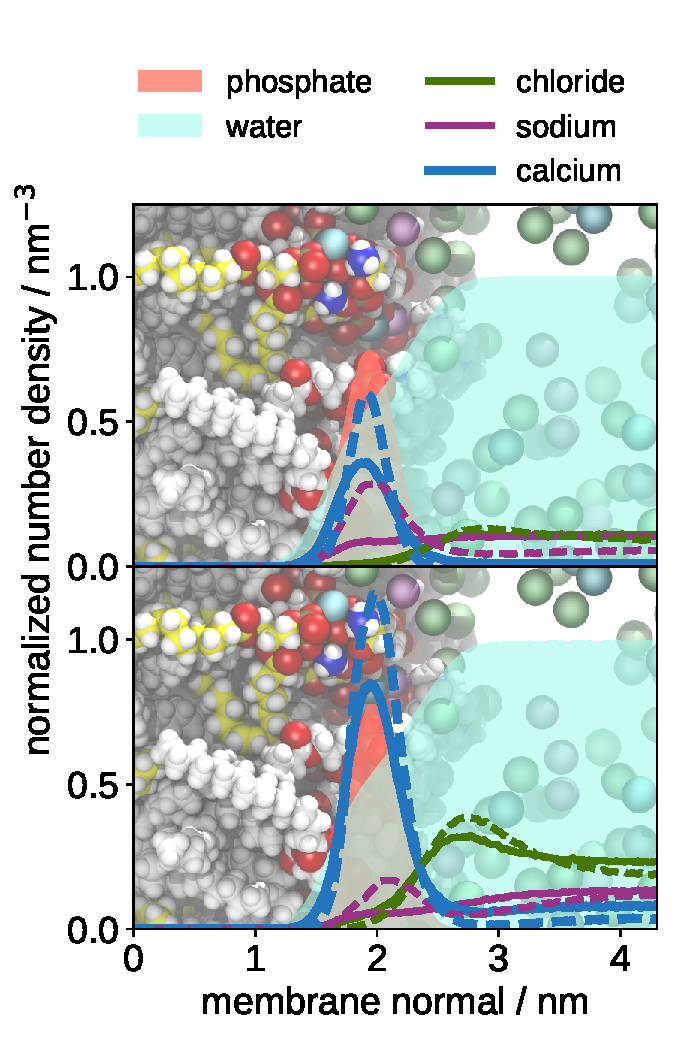
\includegraphics[width=\figwidth]{../img/ecc_pops/density_profiles_ca_na_k_cl_wat_phos_ecclipids_lipid17_compar_80and200mMCaCl2.pdf}
  \caption{\label{fig:cacl-dens_PCPS} 
    Number density profiles of \ce{Ca^{2+}} and \ce{Cl^-} ions and \ce{Na^{+}} counterions 
    along the normal of the membrane starting at the centre
    for the negatively charged membrane with the composition 5\,PC:1\,PS
    at 80~mM (top) and 200~mM (bottom) added buffer concentrations of \ce{CaCl2} from simulations with ECC-lipids (solid) and Lipid17 (dashed). 
    In order to visualize the density profiles with a comparable scale 
    the density profile of~\ce{Ca^{2+}} ions are divided by 2, and 
    the density profiles of phosphate groups and water are divided by 4 and 100, respectively.  
  }
\end{figure} 

%SAMULI: We will not go to the spin relaxation time analysis in this work
%and average angles do not give information about dynamics
%
%It has been pointed out in previous experimental works
%that the conformational flexibility of PS head groups 
%is different from other lipids \cite{browning80}. 
%While the static shielding tensor of PS is not substantially different from PC or PE, 
%the $^{31}$P~$T_1$ relaxation times are significantly shorter for PS. 
%It is suggested that the PS head group is more rigid compared to the other phospholipids, 
%which is also corroborated by a larger chemical shielding anisotropy of PS \cite{browning80}. 

% Description of no. conctacts counting
%Such a significantly increased binding also has an impact 
%on the structure and populations of the bound calcium cations. 
%We have counted contacts between the cations and the oxygen atoms of the lipids
%similarly as was done in \cite{melcr18} 
%to obtain such a detailed information 
%about the interactions of \ce{Ca^{2+}} with various moieties in POPC or POPS. 

% Populations from contacts

Recent analyzes of interaction sites between calcium and PS lipids combining
MD simulations with various experimental techniques have been 
controversial because the results strongly depend on force fields parameters \cite{melcrova16,valentine18,hallock18}.
In ECC-lipids simulation of POPC:POPS (5:1) mixture with 409 mM CaCl$_2$,
the calcium ions bind twice more likely to the carboxylate than to phosphate moiety of POPS headgroup
\todo{I am not sure if this is correct, because I do not understand the numbers in the table.} (Table \ref{tab:binding}),
in line with the results without the NBfix corrections in CHARMM36 \cite{hallock18}.
However, in CHARMM36 simulations without the NBfix correction for calcium,
calcium ions significantly overbind to PC lipids  \cite{catte16} and calcium ions coordinate
with even four distinct PS lipids \cite{hallock18}, while coordination with more than two PS lipids
was not observed in our ECC-lipids simulations (Fig.~\ref{fig:cacl_complexes}).
Furthermore, the POPS:POPC:Ca$^{2+}$ (7:3:7) mixture with relatively high
PS lipid fraction and calcium concentration was used in previous work \cite{hallock18},
which may lead to the complexation of \ce{Ca^{2+}} cations and PS lipids that is
not observed with lower PS content used in ECC-lipids simulations in this work \cite{hauser77,kurland79,hauser85,feigenson86,mattai89,roux90,roux91}.
%While POPC interacts with the calcium cations almost entirely through its phosphate group 
%in both neutral \cite{melcr18} and negatively charged membranes, 
%the inteaction with POPS lipids happens more through the \ce{COO^-} group than through the \ce{PO4} group. 
%Interactions of \ce{Ca^{2+}} with carbonyl groups are also present for both POPC and POPS,
%however, they are always accompanied by interactions with phosphate groups. 
Significant coordination of calcium with carbonyls groups of PS and PC lipids observed in previous
simulations with the Berger force field \cite{melcrova16} %\cite{berger97,mukhopadhyay04}
was not observed in ECC-lipids simulations in here nor in the previous work with pure POPC \cite{melcr18}.
%This is in contrast to 
%combined with fluorescent and vibrational sum frequency spectroscopy,
%which suggest a 
Overestimated coordination of cations with carbonyl groups is a potential source for
overestimated cation binding in Berger force fields \cite{catte16,NMRlipidsIV}. 
In CHARMM36 simulations with the NBfix, calcium mainly interacted with only
carboxylate of PS lipids  \cite{valentine18}, which is a potential source for the
underestimated calcium binding affinity to lipid bilayer with this force field \cite{NMRlipidsIV}. 

%In contrast, the combination of NMR experiments 
%and MD simulations with the same model, CHARMM36, but without the correction for calcium binding
%also reveal long-lived interactions of \ce{Ca^{2+}} with \ce{PO4} groups. \cite{hallock18}
%Although the ratios of the life times of coordination follow the same trends as in our work,
%the lengths of simulation trajectories are insufficient 
%to yield converged results in this aspect (see SI and Refs.~\cite{catte16, melcr18, NMRlipidsIV}). 

\begin{figure}[tb!] 
  \centering 
  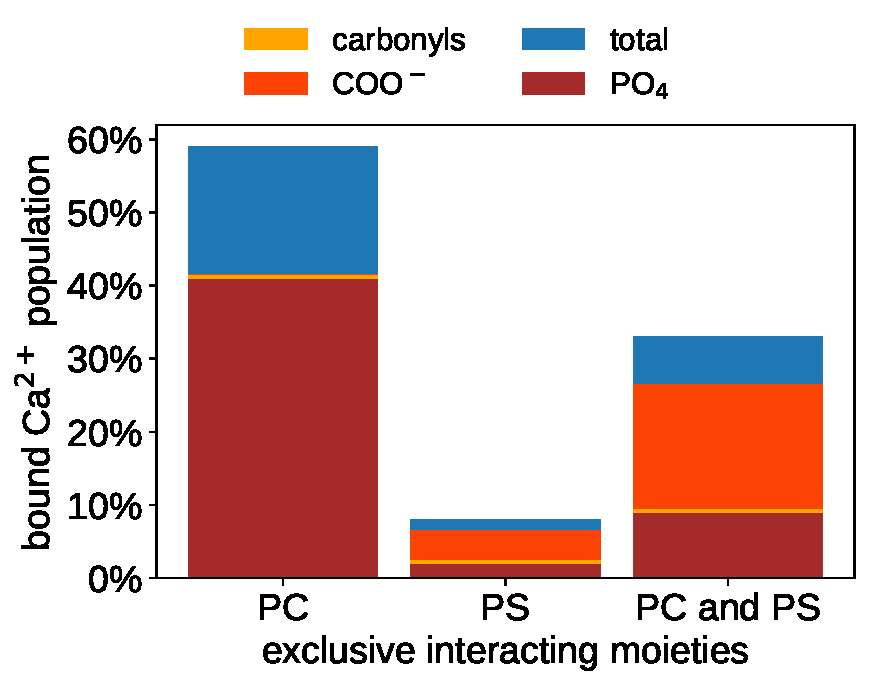
\includegraphics[width=\figwidthsmall]{../img/bound_ca_populations.pdf} 
  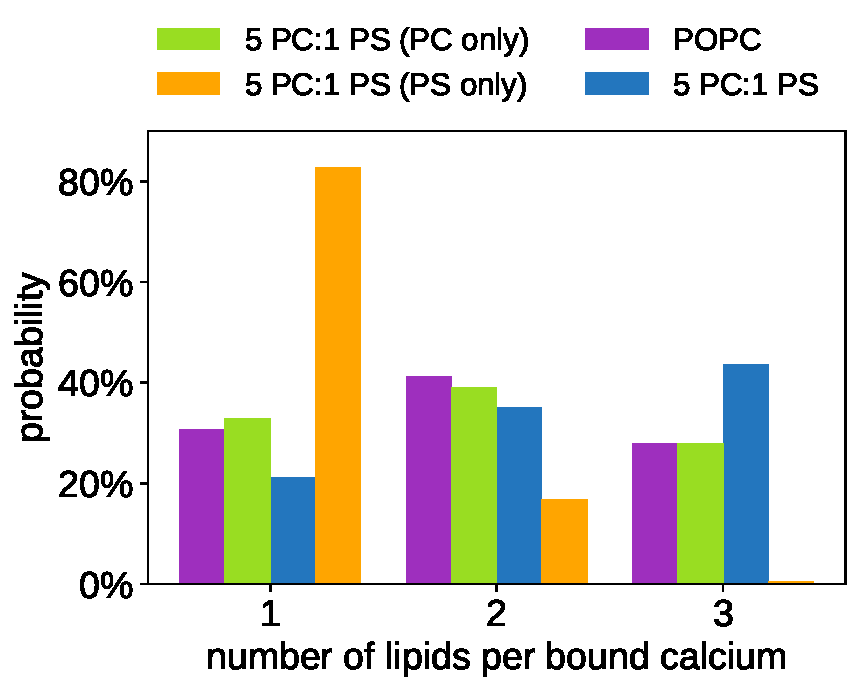
\includegraphics[width=\figwidthsmall]{../img/stoichiometry_CaCl2_comparison_Ecc-lipids_PC-vs-PCPS.pdf} \\ 
  \caption{ \label{fig:cacl_complexes} 
  Left: Percentages of the population of bound Ca$^{2+}$ 
in exclusive contact with various lipid moieties 
in a POPC:POPS (5:1) bilayer with 409 mM CaCl$_2$. 
For comparison, in a pure POPC bilayer with 350 mM CaCl$_2$, 
67\% of bound \ce{Ca^{2+}} is exclusively in contact with \ce{PO_4} group. \cite{melcr18} \\
    Right: Relative probabilities of \ce{Ca^{2+}} ions to coordinate with a certain number of lipids
    in pure POPC bilayer with 350 mM CaCl$_2$ and in POPC:POPS (5:1) mixture with 400 mM CaCl$_2$.  
    Analysis was done for both systems by considering all lipids (blue and violet) and
    for POPC:POPS (5:1) mixture also by considering POPC and POPS lipids separately (green and orange). \\
    %All lipids were taken into account with the exception of the complexes in light green and orange, 
    %for which we counted only contacts with POPC resp POPS from the mixed 5\,PC:1\,PS negatively charged bilayer. 
    %The calculated probabilities of the calcium-lipid complexes also reflect only POPC (light green) resp POPS (orange). 
    % Probabilities were taken from simulations with comparable bulk concentrations of calcium around 250~mM. 
    Clusters of four or more lipids were not observed in either membrane.
    The threshold for counting coordinated lipids in a complex with \ce{Ca^{2+}} was set to $0.3\,\mathrm{nm}$, 
    as the distance between the cation and the oxygen atoms of the lipids. 
    Previously published simulation data \cite{melcr18} for pure POPC bilayers were taken directly from \cite{ECC-POPC_nacl_cacl2_files}. 
  }
\end{figure} 


%Still, the dominant contribution to the binding of calcium comes from the phosphate groups. 
%Interestingly enough,
%although the \ce{COO^-} groups increase the affinity of calcium towards PS compared to PC,
% there is no extra density at the outmost surface of the membrane. 
%This can be understood from the point of the structural rearangements of the \ce{COO^-} group, 
%which take place during the interactions with calcium cations
%described above and in Fig.~\ref{fig:delta_ordPar_CaCl_PCPS}. 

%Simulations using CHARMM36 force field \cite{klauda10,venable13} with
%the NBfix parameters for calcium \cite{kim16}, combined with 2D infrared spectroscopy,
%suggest that calcium ions interact only with the carboxylate group of PS lipids \cite{valentine18}.
%The same force field without the NBfix parameters, combined with NMR chemical shifts and
%rotational-echo double-resonance (REDOR) experiments, suggests a significant binding affinity also to the phosphate region \cite{hallock18}.
%Simulations with the Berger force field \cite{berger97,mukhopadhyay04},
%combined with fluorescent and vibrational sum frequency spectroscopy, suggest a significant
%calcium binding also to the carbonyls in the acyl chains \cite{melcrova16}.

%In PS lipids, the calcium binds both phosphate and carboxylate, but probability for the latter is twice higher.
%In PC lipids, the calcium binds almost always to phosphate, but in some cases also to carbonyl, as also observed previously in pure POPC simulations \cite{melcr18}.

The advantage of the NMR order parameters used in this work is the direct connection between
measured and simulation data, which enables more unambiguous evaluation of the force field quality \cite{catte16,ollila16}
than more indirect comparison in previous studies using 2D infrared spectroscopy \cite{valentine18}, NMR chemical shifts and
rotational-echo double-resonance (REDOR) experiments \cite{hallock18} or fluorescent and vibrational sum frequency spectroscopy \cite{melcrova16}.
Because the ECC-lipids model gives the best agreement with the experimental headgroup order parameters
with various ion conctenrations among the available models, we believe that it gives the currently best available
interpretation of the experimental data. Athough the ECC-lipids model gives the most realistic picture of calcium binding to
lipid bilayers containing PS lipids with respect to NMR order parameters, it does not
correctly capture the rapid changes with small concentrations. Therefore, further
force field optimization is required for fully realistic MD simulations of cations
in the vicinity of negatively charged lipid bilayers.

%Despite significant improvements in the ECC-lipid against Lipid17/Dang
%and other force fields for the response of PS headgroup order parameters to
%the bound calcium \cite{NMRlipidsIV}, 
%the model (Fig.~\ref{fig:delta_ordPar_CaCl_PCPS}).

% and also possibly from the approximate mean-field treatment of the electronic polarization. 


%
% SAMULI: We have problems to find time to finish this paper even with the current data, we should not add anything that is not necessary to finish this asap. 
%
%\todo{JOE: suggestion -- what is the charge at the membrane interface of memb+counterions -vs- memb+CaCl2 concnetration?
% this could relate well to the zeta potential measurements and the Fig 1 in \cite{melcrova16}. }
% 
%\todo{ THE REMAINING PIECES TO BE DISCUSSED  --  consider wheter the dynamics slowdown or the dihedral distributions could make good contributions to this paper. }


%% Ca2+ induces much slower dynamics of lipids when PS is present,
%% this does not happen with PC
%% uses NBFIX
%From Ref.~\cite{valentine18}://
%To summarize, calcium binding to PS lipids slows the dynamics at the ester position and introduces more heterogeneous molecular environments. 
%The slowdown cannot be attributed to complete ester dehydration or decreased hydrogen bonding to water, so we interpret these results as evidence that the lipid headgroups adopt more rigid but %disordered conformations on the molecular level. 
%The decrease in dynamics observed experimentally indicates that the network of hydrogen bonds between lipids and water at the polar-nonpolar interface becomes slower, as it was shown by Karatha%nou and Bondar (34). 
%This is bolstered by recent NMR work showing that binding to Ca2+ induces two different rigid conformations in the glycerol backbone of lipid headgroups (18).
%We have investigated the molecular origin of the rigidification and decreased lateral diffusion, finding that calcium binding does not dehydrate the ester region, but even with only 10\% PS lip%ids, the local dynamics slow around the esters. The slower local dynamics provide a molecular explanation for the Ca2+-dependent decreases in fluidity observed on longer length and timescales.
%There is considerable room for further improvement in the force fields for ion-membrane interactions. Particularly, small differences in short-range interactions may determine the local geometr%ies (34
%). Most of our conclusions are, however, based on long-range effects (i.e., electric field generated by the ion at significant distances from the carbonyl groups), which are less sensitive to t%he details of the force field. 



%Their Figure 5 \cite{hallock18} shows the distributions of O-Ca-Cb-N dihedral angle
%revealing separate populations of the PS head groups. 
%These two structures are also compared in therm of P-Cg distances, 
%which can be measured from NMR REDOR exp. 
%It is concluded that since the two distinct populations in P-Cg distance can be represented with the 
%dihedral distributions, 
%they also likely represent the distinct populations. 
% -> plotting the distribution of O-Ca-Cb-N dihedral angle may be also a good idea for us (SI?)
%     -> NMRlipids 4 in SI \cite{NMRlipidsIV} plots this information: 
%           - C36 agress with the distribution in \cite{hallock18}
%           - Lipid17 (and Slipids) are almost identical to C36
%           - but the structure of the COO- is highly different (dih angle Ca-Cb-Cg-Og)

 
\section{Conclusions} 

\todo{SAMULI: I have putted here two preliminary sentences
JOSEF: I can write conclusions, but I would prefer to wait with that after your comments and edits. }
Applying ECC to POPS lipids improves cation binding affinity to membranes
mixed with POPC and also the response of PS headgroup to the bound cations.
However, further improvement of the parameters is needed to fully reproduce the
details of calcium binding to PS headgroups.



\listoftodos


% If you have acknowledgments, this puts in the proper section head. 
\begin{acknowledgement} 
% Put your acknowledgments here. 
P.J. acknowledges support from the Czech Science Foundation (grant no. 16-01074S)  
and from the Academy of Finland via the FiDiPro award. 
Computational resources were supplied by the Ministry of Education, Youth and Sports 
of the Czech Republic under the Projects CESNET (Project No. LM2015042) and CERIT-Scientific 
Cloud (Project No. LM2015085) provided within the program Projects of Large Research, 
Development and Innovations Infrastructures. 
O.H.S.O. acknowledges financial support from 
Integrated Structural Biology Research Infrastructure of 
Helsinki Institute of Life Science (Instruct-HiLIFE). 
\end{acknowledgement} 
 
\begin{suppinfo} 
 
%A listing of the contents of each file supplied as Supporting Information 
%should be included. For instructions on what should be included in the 
%Supporting Information as well as how to prepare this material for 
%publications, refer to the journal's Instructions for Authors. 
 
%The following files are available free of charge. 
%\begin{itemize} 
%  \item Filename: brief description 
%\end{itemize} 
 
\end{suppinfo} 
 
 
\bibliography{refs.bib} 
 
\end{document} 
 

